% Created 2022-09-04 Sun 21:49
% Intended LaTeX compiler: pdflatex
\documentclass[11pt]{article}
\usepackage[utf8]{inputenc}
\usepackage[T1]{fontenc}
\usepackage{graphicx}
\usepackage{longtable}
\usepackage{wrapfig}
\usepackage{rotating}
\usepackage[normalem]{ulem}
\usepackage{amsmath}
\usepackage{amssymb}
\usepackage{capt-of}
\usepackage{hyperref}
\graphicspath{{../../books/}}
% wrong resolution of image
% https://tex.stackexchange.com/questions/21627/image-from-includegraphics-showing-in-wrong-image-size?rq=1

%%%%%%%%%%%%%%%%%%%%%%%%%%%%%%%%%%%%%%
%% TIPS                                 %%
%%%%%%%%%%%%%%%%%%%%%%%%%%%%%%%%%%%%%%
% \substack{a\\b} for multiple lines text
% \usepackage{expl3}
% \expandafter\def\csname ver@l3regex.sty\endcsname{}
% \usepackage{pkgloader}
\usepackage[utf8]{inputenc}

% nfss error
% \usepackage[B1,T1]{fontenc}
\usepackage{fontspec}

% \usepackage[Emoticons]{ucharclasses}
\newfontfamily\DejaSans{DejaVu Sans}
% \setDefaultTransitions{\DejaSans}{}

% pdfplots will load xolor automatically without option
\usepackage[dvipsnames]{xcolor}

%                                                             ┳┳┓   ┓
%                                                             ┃┃┃┏┓╋┣┓
%                                                             ┛ ┗┗┻┗┛┗
% \usepackage{amsmath} mathtools loads the amsmath
\usepackage{amsmath}
\usepackage{mathtools}

\usepackage{amsthm}
\usepackage{amsbsy}

%\usepackage{commath}

\usepackage{amssymb}

\usepackage{mathrsfs}
%\usepackage{mathabx}
\usepackage{stmaryrd}
\usepackage{empheq}

\usepackage{scalerel}
\usepackage{stackengine}
\usepackage{stackrel}



\usepackage{nicematrix}
\usepackage{tensor}
\usepackage{blkarray}
\usepackage{siunitx}
\usepackage[f]{esvect}

% centering \not on a letter
\usepackage{slashed}
\usepackage[makeroom]{cancel}

%\usepackage{merriweather}
\usepackage{unicode-math}
\setmainfont{TeX Gyre Pagella}
% \setmathfont{STIX}
%\setmathfont{texgyrepagella-math.otf}
%\setmathfont{Libertinus Math}
\setmathfont{Latin Modern Math}

 % \setmathfont[range={\smwhtdiamond,\enclosediamond,\varlrtriangle}]{Latin Modern Math}
\setmathfont[range={\rightrightarrows,\twoheadrightarrow,\leftrightsquigarrow,\triangledown,\vartriangle,\precneq,\succneq,\prec,\succ,\preceq,\succeq,\tieconcat}]{XITS Math}
 \setmathfont[range={\int,\setminus}]{Libertinus Math}
 % \setmathfont[range={\mathalpha}]{TeX Gyre Pagella Math}
%\setmathfont[range={\mitA,\mitB,\mitC,\mitD,\mitE,\mitF,\mitG,\mitH,\mitI,\mitJ,\mitK,\mitL,\mitM,\mitN,\mitO,\mitP,\mitQ,\mitR,\mitS,\mitT,\mitU,\mitV,\mitW,\mitX,\mitY,\mitZ,\mita,\mitb,\mitc,\mitd,\mite,\mitf,\mitg,\miti,\mitj,\mitk,\mitl,\mitm,\mitn,\mito,\mitp,\mitq,\mitr,\mits,\mitt,\mitu,\mitv,\mitw,\mitx,\mity,\mitz}]{TeX Gyre Pagella Math}
% unicode is not good at this!
%\let\nmodels\nvDash

 \usepackage{wasysym}

 % for wide hat
 \DeclareSymbolFont{yhlargesymbols}{OMX}{yhex}{m}{n} \DeclareMathAccent{\what}{\mathord}{yhlargesymbols}{"62}

%                                                               ┏┳┓•┓
%                                                                ┃ ┓┃┏┓
%                                                                ┻ ┗┛┗┗

\usepackage{pgfplots}
\pgfplotsset{compat=1.18}
\usepackage{tikz}
\usepackage{tikz-cd}
\tikzcdset{scale cd/.style={every label/.append style={scale=#1},
    cells={nodes={scale=#1}}}}
% TODO: discard qtree and use forest
% \usepackage{tikz-qtree}
\usepackage{forest}

\usetikzlibrary{arrows,positioning,calc,fadings,decorations,matrix,decorations,shapes.misc}
%setting from geogebra
\definecolor{ccqqqq}{rgb}{0.8,0,0}

%                                                          ┳┳┓•    ┓┓
%                                                          ┃┃┃┓┏┏┏┓┃┃┏┓┏┓┏┓┏┓┓┏┏
%                                                          ┛ ┗┗┛┗┗ ┗┗┗┻┛┗┗ ┗┛┗┻┛
%\usepackage{twemojis}
\usepackage[most]{tcolorbox}
\usepackage{threeparttable}
\usepackage{tabularx}

\usepackage{enumitem}
\usepackage[indLines=false]{algpseudocodex}
\usepackage[]{algorithm2e}
% \SetKwComment{Comment}{/* }{ */}
% \algrenewcommand\algorithmicrequire{\textbf{Input:}}
% \algrenewcommand\algorithmicensure{\textbf{Output:}}
% wrong with preview
\usepackage{subcaption}
\usepackage{caption}
% {\aunclfamily\Huge}
\usepackage{auncial}

\usepackage{float}

\usepackage{fancyhdr}

\usepackage{ifthen}
\usepackage{xargs}

\definecolor{mintedbg}{rgb}{0.99,0.99,0.99}
\usepackage[cachedir=\detokenize{~/miscellaneous/trash}]{minted}
\setminted{breaklines,
  mathescape,
  bgcolor=mintedbg,
  fontsize=\footnotesize,
  frame=single,
  linenos}
\usemintedstyle{xcode}
\usepackage{tcolorbox}
\usepackage{etoolbox}



\usepackage{imakeidx}
\usepackage{hyperref}
\usepackage{soul}
\usepackage{framed}

% don't use this for preview
%\usepackage[margin=1.5in]{geometry}
% \usepackage{geometry}
% \geometry{legalpaper, landscape, margin=1in}
\usepackage[font=itshape]{quoting}

%\LoadPackagesNow
%\usepackage[xetex]{preview}
%%%%%%%%%%%%%%%%%%%%%%%%%%%%%%%%%%%%%%%
%% USEPACKAGES end                       %%
%%%%%%%%%%%%%%%%%%%%%%%%%%%%%%%%%%%%%%%

%%%%%%%%%%%%%%%%%%%%%%%%%%%%%%%%%%%%%%%
%% Algorithm environment
%%%%%%%%%%%%%%%%%%%%%%%%%%%%%%%%%%%%%%%
\SetKwIF{Recv}{}{}{upon receiving}{do}{}{}{}
\SetKwBlock{Init}{initially do}{}
\SetKwProg{Function}{Function}{:}{}

% https://github.com/chrmatt/algpseudocodex/issues/3
\algnewcommand\algorithmicswitch{\textbf{switch}}%
\algnewcommand\algorithmiccase{\textbf{case}}
\algnewcommand\algorithmicof{\textbf{of}}
\algnewcommand\algorithmicotherwise{\texttt{otherwise} $\Rightarrow$}

\makeatletter
\algdef{SE}[SWITCH]{Switch}{EndSwitch}[1]{\algpx@startIndent\algpx@startCodeCommand\algorithmicswitch\ #1\ \algorithmicdo}{\algpx@endIndent\algpx@startCodeCommand\algorithmicend\ \algorithmicswitch}%
\algdef{SE}[CASE]{Case}{EndCase}[1]{\algpx@startIndent\algpx@startCodeCommand\algorithmiccase\ #1}{\algpx@endIndent\algpx@startCodeCommand\algorithmicend\ \algorithmiccase}%
\algdef{SE}[CASEOF]{CaseOf}{EndCaseOf}[1]{\algpx@startIndent\algpx@startCodeCommand\algorithmiccase\ #1 \algorithmicof}{\algpx@endIndent\algpx@startCodeCommand\algorithmicend\ \algorithmiccase}
\algdef{SE}[OTHERWISE]{Otherwise}{EndOtherwise}[0]{\algpx@startIndent\algpx@startCodeCommand\algorithmicotherwise}{\algpx@endIndent\algpx@startCodeCommand\algorithmicend\ \algorithmicotherwise}
\ifbool{algpx@noEnd}{%
  \algtext*{EndSwitch}%
  \algtext*{EndCase}%
  \algtext*{EndCaseOf}
  \algtext*{EndOtherwise}
  %
  % end indent line after (not before), to get correct y position for multiline text in last command
  \apptocmd{\EndSwitch}{\algpx@endIndent}{}{}%
  \apptocmd{\EndCase}{\algpx@endIndent}{}{}%
  \apptocmd{\EndCaseOf}{\algpx@endIndent}{}{}
  \apptocmd{\EndOtherwise}{\algpx@endIndent}{}{}
}{}%

\pretocmd{\Switch}{\algpx@endCodeCommand}{}{}
\pretocmd{\Case}{\algpx@endCodeCommand}{}{}
\pretocmd{\CaseOf}{\algpx@endCodeCommand}{}{}
\pretocmd{\Otherwise}{\algpx@endCodeCommand}{}{}

% for end commands that may not be printed, tell endCodeCommand whether we are using noEnd
\ifbool{algpx@noEnd}{%
  \pretocmd{\EndSwitch}{\algpx@endCodeCommand[1]}{}{}%
  \pretocmd{\EndCase}{\algpx@endCodeCommand[1]}{}{}
  \pretocmd{\EndCaseOf}{\algpx@endCodeCommand[1]}{}{}%
  \pretocmd{\EndOtherwise}{\algpx@endCodeCommand[1]}{}{}
}{%
  \pretocmd{\EndSwitch}{\algpx@endCodeCommand[0]}{}{}%
  \pretocmd{\EndCase}{\algpx@endCodeCommand[0]}{}{}%
  \pretocmd{\EndCaseOf}{\algpx@endCodeCommand[0]}{}{}
  \pretocmd{\EndOtherwise}{\algpx@endCodeCommand[0]}{}{}
}%
\makeatother
% % For algpseudocode
% \algnewcommand\algorithmicswitch{\textbf{switch}}
% \algnewcommand\algorithmiccase{\textbf{case}}
% \algnewcommand\algorithmiccaseof{\textbf{case}}
% \algnewcommand\algorithmicof{\textbf{of}}
% % New "environments"
% \algdef{SE}[SWITCH]{Switch}{EndSwitch}[1]{\algorithmicswitch\ #1\ \algorithmicdo}{\algorithmicend\ \algorithmicswitch}%
% \algdef{SE}[CASE]{Case}{EndCase}[1]{\algorithmiccase\ #1}{\algorithmicend\ \algorithmiccase}%
% \algtext*{EndSwitch}%
% \algtext*{EndCase}
% \algdef{SE}[CASEOF]{CaseOf}{EndCaseOf}[1]{\algorithmiccaseof\ #1 \algorithmicof}{\algorithmicend\ \algorithmiccaseof}
% \algtext*{EndCaseOf}



%\pdfcompresslevel0

% quoting from
% https://tex.stackexchange.com/questions/391726/the-quotation-environment
\NewDocumentCommand{\bywhom}{m}{% the Bourbaki trick
  {\nobreak\hfill\penalty50\hskip1em\null\nobreak
   \hfill\mbox{\normalfont(#1)}%
   \parfillskip=0pt \finalhyphendemerits=0 \par}%
}

\NewDocumentEnvironment{pquotation}{m}
  {\begin{quoting}[
     indentfirst=true,
     leftmargin=\parindent,
     rightmargin=\parindent]\itshape}
  {\bywhom{#1}\end{quoting}}

\indexsetup{othercode=\small}
\makeindex[columns=2,options={-s /media/wu/file/stuuudy/notes/index_style.ist},intoc]
\makeatletter
\def\@idxitem{\par\hangindent 0pt}
\makeatother


% \newcounter{dummy} \numberwithin{dummy}{section}
\newtheorem{dummy}{dummy}[section]
\theoremstyle{definition}
\newtheorem{definition}[dummy]{Definition}
\theoremstyle{plain}
\newtheorem{corollary}[dummy]{Corollary}
\newtheorem{lemma}[dummy]{Lemma}
\newtheorem{proposition}[dummy]{Proposition}
\newtheorem{theorem}[dummy]{Theorem}
\newtheorem{notation}[dummy]{Notation}
\newtheorem{conjecture}[dummy]{Conjecture}
\newtheorem{fact}[dummy]{Fact}
\newtheorem{warning}[dummy]{Warning}
\theoremstyle{definition}
\newtheorem{examplle}{Example}[section]
\theoremstyle{remark}
\newtheorem*{remark}{Remark}
\newtheorem{exercise}{Exercise}[subsection]
\newtheorem{problem}{Problem}[subsection]
\newtheorem{observation}{Observation}[section]
\newenvironment{claim}[1]{\par\noindent\textbf{Claim:}\space#1}{}

\makeatletter
\DeclareFontFamily{U}{tipa}{}
\DeclareFontShape{U}{tipa}{m}{n}{<->tipa10}{}
\newcommand{\arc@char}{{\usefont{U}{tipa}{m}{n}\symbol{62}}}%

\newcommand{\arc}[1]{\mathpalette\arc@arc{#1}}

\newcommand{\arc@arc}[2]{%
  \sbox0{$\m@th#1#2$}%
  \vbox{
    \hbox{\resizebox{\wd0}{\height}{\arc@char}}
    \nointerlineskip
    \box0
  }%
}
\makeatother

\setcounter{MaxMatrixCols}{20}
%%%%%%% ABS
\DeclarePairedDelimiter\abss{\lvert}{\rvert}%
\DeclarePairedDelimiter\normm{\lVert}{\rVert}%

% Swap the definition of \abs* and \norm*, so that \abs
% and \norm resizes the size of the brackets, and the
% starred version does not.
\makeatletter
\let\oldabs\abss
%\def\abs{\@ifstar{\oldabs}{\oldabs*}}
\newcommand{\abs}{\@ifstar{\oldabs}{\oldabs*}}
\newcommand{\norm}[1]{\left\lVert#1\right\rVert}
%\let\oldnorm\normm
%\def\norm{\@ifstar{\oldnorm}{\oldnorm*}}
%\renewcommand{norm}{\@ifstar{\oldnorm}{\oldnorm*}}
\makeatother

% \stackMath
% \newcommand\what[1]{%
% \savestack{\tmpbox}{\stretchto{%
%   \scaleto{%
%     \scalerel*[\widthof{\ensuremath{#1}}]{\kern-.6pt\bigwedge\kern-.6pt}%
%     {\rule[-\textheight/2]{1ex}{\textheight}}%WIDTH-LIMITED BIG WEDGE
%   }{\textheight}%
% }{0.5ex}}%
% \stackon[1pt]{#1}{\tmpbox}%
% }

% \newcommand\what[1]{\ThisStyle{%
%     \setbox0=\hbox{$\SavedStyle#1$}%
%     \stackengine{-1.0\ht0+.5pt}{$\SavedStyle#1$}{%
%       \stretchto{\scaleto{\SavedStyle\mkern.15mu\char'136}{2.6\wd0}}{1.4\ht0}%
%     }{O}{c}{F}{T}{S}%
%   }
% }

% \newcommand\wtilde[1]{\ThisStyle{%
%     \setbox0=\hbox{$\SavedStyle#1$}%
%     \stackengine{-.1\LMpt}{$\SavedStyle#1$}{%
%       \stretchto{\scaleto{\SavedStyle\mkern.2mu\AC}{.5150\wd0}}{.6\ht0}%
%     }{O}{c}{F}{T}{S}%
%   }
% }

% \newcommand\wbar[1]{\ThisStyle{%
%     \setbox0=\hbox{$\SavedStyle#1$}%
%     \stackengine{.5pt+\LMpt}{$\SavedStyle#1$}{%
%       \rule{\wd0}{\dimexpr.3\LMpt+.3pt}%
%     }{O}{c}{F}{T}{S}%
%   }
% }

\newcommand{\bl}[1] {\boldsymbol{#1}}
\newcommand{\Wt}[1] {\stackrel{\sim}{\smash{#1}\rule{0pt}{1.1ex}}}
\newcommand{\wt}[1] {\widetilde{#1}}
\newcommand{\tf}[1] {\textbf{#1}}

\newcommand{\wu}[1]{{\color{red} #1}}

%For boxed texts in align, use Aboxed{}
%otherwise use boxed{}

\DeclareMathSymbol{\widehatsym}{\mathord}{largesymbols}{"62}
\newcommand\lowerwidehatsym{%
  \text{\smash{\raisebox{-1.3ex}{%
    $\widehatsym$}}}}
\newcommand\fixwidehat[1]{%
  \mathchoice
    {\accentset{\displaystyle\lowerwidehatsym}{#1}}
    {\accentset{\textstyle\lowerwidehatsym}{#1}}
    {\accentset{\scriptstyle\lowerwidehatsym}{#1}}
    {\accentset{\scriptscriptstyle\lowerwidehatsym}{#1}}
  }


\newcommand{\cupdot}{\mathbin{\dot{\cup}}}
\newcommand{\bigcupdot}{\mathop{\dot{\bigcup}}}

\usepackage{graphicx}

\usepackage[toc,page]{appendix}

% text on arrow for xRightarrow
\makeatletter
%\newcommand{\xRightarrow}[2][]{\ext@arrow 0359\Rightarrowfill@{#1}{#2}}
\makeatother

% Arbitrary long arrow
\newcommand{\Rarrow}[1]{%
\parbox{#1}{\tikz{\draw[->](0,0)--(#1,0);}}
}

\newcommand{\LRarrow}[1]{%
\parbox{#1}{\tikz{\draw[<->](0,0)--(#1,0);}}
}


\makeatletter
\providecommand*{\rmodels}{%
  \mathrel{%
    \mathpalette\@rmodels\models
  }%
}
\newcommand*{\@rmodels}[2]{%
  \reflectbox{$\m@th#1#2$}%
}
\makeatother

% Roman numerals
\makeatletter
\newcommand*{\rom}[1]{\expandafter\@slowromancap\romannumeral #1@}
\makeatother
% \\def \\b\([a-zA-Z]\) {\\boldsymbol{[a-zA-z]}}
% \\DeclareMathOperator{\\b\1}{\\textbf{\1}}

\DeclareMathOperator*{\argmin}{arg\,min}
\DeclareMathOperator*{\argmax}{arg\,max}

\DeclareMathOperator{\bone}{\textbf{1}}
\DeclareMathOperator{\bx}{\textbf{x}}
\DeclareMathOperator{\bz}{\textbf{z}}
\DeclareMathOperator{\bff}{\textbf{f}}
\DeclareMathOperator{\ba}{\textbf{a}}
\DeclareMathOperator{\bk}{\textbf{k}}
\DeclareMathOperator{\bs}{\textbf{s}}
\DeclareMathOperator{\bh}{\textbf{h}}
\DeclareMathOperator{\bc}{\textbf{c}}
\DeclareMathOperator{\br}{\textbf{r}}
\DeclareMathOperator{\bi}{\textbf{i}}
\DeclareMathOperator{\bj}{\textbf{j}}
\DeclareMathOperator{\bn}{\textbf{n}}
\DeclareMathOperator{\be}{\textbf{e}}
\DeclareMathOperator{\bo}{\textbf{o}}
\DeclareMathOperator{\bU}{\textbf{U}}
\DeclareMathOperator{\bL}{\textbf{L}}
\DeclareMathOperator{\bV}{\textbf{V}}
\def \bzero {\mathbf{0}}
\def \bbone {\mathbb{1}}
\def \btwo {\mathbf{2}}
\DeclareMathOperator{\bv}{\textbf{v}}
\DeclareMathOperator{\bp}{\textbf{p}}
\DeclareMathOperator{\bI}{\textbf{I}}
\def \dbI {\dot{\bI}}
\DeclareMathOperator{\bM}{\textbf{M}}
\DeclareMathOperator{\bN}{\textbf{N}}
\DeclareMathOperator{\bK}{\textbf{K}}
\DeclareMathOperator{\bt}{\textbf{t}}
\DeclareMathOperator{\bb}{\textbf{b}}
\DeclareMathOperator{\bA}{\textbf{A}}
\DeclareMathOperator{\bX}{\textbf{X}}
\DeclareMathOperator{\bu}{\textbf{u}}
\DeclareMathOperator{\bS}{\textbf{S}}
\DeclareMathOperator{\bZ}{\textbf{Z}}
\DeclareMathOperator{\bJ}{\textbf{J}}
\DeclareMathOperator{\by}{\textbf{y}}
\DeclareMathOperator{\bw}{\textbf{w}}
\DeclareMathOperator{\bT}{\textbf{T}}
\DeclareMathOperator{\bF}{\textbf{F}}
\DeclareMathOperator{\bmm}{\textbf{m}}
\DeclareMathOperator{\bW}{\textbf{W}}
\DeclareMathOperator{\bR}{\textbf{R}}
\DeclareMathOperator{\bC}{\textbf{C}}
\DeclareMathOperator{\bD}{\textbf{D}}
\DeclareMathOperator{\bE}{\textbf{E}}
\DeclareMathOperator{\bQ}{\textbf{Q}}
\DeclareMathOperator{\bP}{\textbf{P}}
\DeclareMathOperator{\bY}{\textbf{Y}}
\DeclareMathOperator{\bH}{\textbf{H}}
\DeclareMathOperator{\bB}{\textbf{B}}
\DeclareMathOperator{\bG}{\textbf{G}}
\def \blambda {\symbf{\lambda}}
\def \boldeta {\symbf{\eta}}
\def \balpha {\symbf{\alpha}}
\def \btau {\symbf{\tau}}
\def \bbeta {\symbf{\beta}}
\def \bgamma {\symbf{\gamma}}
\def \bxi {\symbf{\xi}}
\def \bLambda {\symbf{\Lambda}}
\def \bGamma {\symbf{\Gamma}}

\newcommand{\bto}{{\boldsymbol{\to}}}
\newcommand{\Ra}{\Rightarrow}
\newcommand{\xrsa}[1]{\overset{#1}{\rightsquigarrow}}
\newcommand{\xlsa}[1]{\overset{#1}{\leftsquigarrow}}
\newcommand\und[1]{\underline{#1}}
\newcommand\ove[1]{\overline{#1}}
%\def \concat {\verb|^|}
\def \bPhi {\mbfPhi}
\def \btheta {\mbftheta}
\def \bTheta {\mbfTheta}
\def \bmu {\mbfmu}
\def \bphi {\mbfphi}
\def \bSigma {\mbfSigma}
\def \la {\langle}
\def \ra {\rangle}

\def \caln {\mathcal{N}}
\def \dissum {\displaystyle\Sigma}
\def \dispro {\displaystyle\prod}

\def \caret {\verb!^!}

\def \A {\mathbb{A}}
\def \B {\mathbb{B}}
\def \C {\mathbb{C}}
\def \D {\mathbb{D}}
\def \E {\mathbb{E}}
\def \F {\mathbb{F}}
\def \G {\mathbb{G}}
\def \H {\mathbb{H}}
\def \I {\mathbb{I}}
\def \J {\mathbb{J}}
\def \K {\mathbb{K}}
\def \L {\mathbb{L}}
\def \M {\mathbb{M}}
\def \N {\mathbb{N}}
\def \O {\mathbb{O}}
\def \P {\mathbb{P}}
\def \Q {\mathbb{Q}}
\def \R {\mathbb{R}}
\def \S {\mathbb{S}}
\def \T {\mathbb{T}}
\def \U {\mathbb{U}}
\def \V {\mathbb{V}}
\def \W {\mathbb{W}}
\def \X {\mathbb{X}}
\def \Y {\mathbb{Y}}
\def \Z {\mathbb{Z}}

\def \cala {\mathcal{A}}
\def \cale {\mathcal{E}}
\def \calb {\mathcal{B}}
\def \calq {\mathcal{Q}}
\def \calp {\mathcal{P}}
\def \cals {\mathcal{S}}
\def \calx {\mathcal{X}}
\def \caly {\mathcal{Y}}
\def \calg {\mathcal{G}}
\def \cald {\mathcal{D}}
\def \caln {\mathcal{N}}
\def \calr {\mathcal{R}}
\def \calt {\mathcal{T}}
\def \calm {\mathcal{M}}
\def \calw {\mathcal{W}}
\def \calc {\mathcal{C}}
\def \calv {\mathcal{V}}
\def \calf {\mathcal{F}}
\def \calk {\mathcal{K}}
\def \call {\mathcal{L}}
\def \calu {\mathcal{U}}
\def \calo {\mathcal{O}}
\def \calh {\mathcal{H}}
\def \cali {\mathcal{I}}
\def \calj {\mathcal{J}}

\def \bcup {\bigcup}

% set theory

\def \zfcc {\textbf{ZFC}^-}
\def \BGC {\textbf{BGC}}
\def \BG {\textbf{BG}}
\def \ac  {\textbf{AC}}
\def \gl  {\textbf{L }}
\def \gll {\textbf{L}}
\newcommand{\zfm}{$\textbf{ZF}^-$}

\def \ZFm {\text{ZF}^-}
\def \ZFCm {\text{ZFC}^-}
\DeclareMathOperator{\WF}{WF}
\DeclareMathOperator{\On}{On}
\def \on {\textbf{On }}
\def \cm {\textbf{M }}
\def \cn {\textbf{N }}
\def \cv {\textbf{V }}
\def \zc {\textbf{ZC }}
\def \zcm {\textbf{ZC}}
\def \zff {\textbf{ZF}}
\def \wfm {\textbf{WF}}
\def \onm {\textbf{On}}
\def \cmm {\textbf{M}}
\def \cnm {\textbf{N}}
\def \cvm {\textbf{V}}

\renewcommand{\restriction}{\mathord{\upharpoonright}}
%% another restriction
\newcommand\restr[2]{{% we make the whole thing an ordinary symbol
  \left.\kern-\nulldelimiterspace % automatically resize the bar with \right
  #1 % the function
  \vphantom{\big|} % pretend it's a little taller at normal size
  \right|_{#2} % this is the delimiter
  }}

\def \pred {\text{pred}}

\def \rank {\text{rank}}
\def \Con {\text{Con}}
\def \deff {\text{Def}}


\def \uin {\underline{\in}}
\def \oin {\overline{\in}}
\def \uR {\underline{R}}
\def \oR {\overline{R}}
\def \uP {\underline{P}}
\def \oP {\overline{P}}

\def \dsum {\displaystyle\sum}

\def \Ra {\Rightarrow}

\def \e {\enspace}

\def \sgn {\operatorname{sgn}}
\def \gen {\operatorname{gen}}
\def \Hom {\operatorname{Hom}}
\def \hom {\operatorname{hom}}
\def \Sub {\operatorname{Sub}}

\def \supp {\operatorname{supp}}

\def \epiarrow {\twoheadarrow}
\def \monoarrow {\rightarrowtail}
\def \rrarrow {\rightrightarrows}

% \def \minus {\text{-}}
% \newcommand{\minus}{\scalebox{0.75}[1.0]{$-$}}
% \DeclareUnicodeCharacter{002D}{\minus}


\def \tril {\triangleleft}

\def \ISigma {\text{I}\Sigma}
\def \IDelta {\text{I}\Delta}
\def \IPi {\text{I}\Pi}
\def \ACF {\textsf{ACF}}
\def \pCF {\textit{p}\text{CF}}
\def \ACVF {\textsf{ACVF}}
\def \HLR {\textsf{HLR}}
\def \OAG {\textsf{OAG}}
\def \RCF {\textsf{RCF}}
\DeclareMathOperator{\GL}{GL}
\DeclareMathOperator{\PGL}{PGL}
\DeclareMathOperator{\SL}{SL}
\DeclareMathOperator{\Inv}{Inv}
\DeclareMathOperator{\res}{res}
\DeclareMathOperator{\Sym}{Sym}
%\DeclareMathOperator{\char}{char}
\def \equal {=}

\def \degree {\text{degree}}
\def \app {\text{App}}
\def \FV {\text{FV}}
\def \conv {\text{conv}}
\def \cont {\text{cont}}
\DeclareMathOperator{\cl}{\text{cl}}
\DeclareMathOperator{\trcl}{\text{trcl}}
\DeclareMathOperator{\sg}{sg}
\DeclareMathOperator{\trdeg}{trdeg}
\def \Ord {\text{Ord}}

\DeclareMathOperator{\cf}{cf}
\DeclareMathOperator{\zfc}{ZFC}

%\DeclareMathOperator{\Th}{Th}
%\def \th {\text{Th}}
% \newcommand{\th}{\text{Th}}
\DeclareMathOperator{\type}{type}
\DeclareMathOperator{\zf}{\textbf{ZF}}
\def \fa {\mathfrak{a}}
\def \fb {\mathfrak{b}}
\def \fc {\mathfrak{c}}
\def \fd {\mathfrak{d}}
\def \fe {\mathfrak{e}}
\def \ff {\mathfrak{f}}
\def \fg {\mathfrak{g}}
\def \fh {\mathfrak{h}}
%\def \fi {\mathfrak{i}}
\def \fj {\mathfrak{j}}
\def \fk {\mathfrak{k}}
\def \fl {\mathfrak{l}}
\def \fm {\mathfrak{m}}
\def \fn {\mathfrak{n}}
\def \fo {\mathfrak{o}}
\def \fp {\mathfrak{p}}
\def \fq {\mathfrak{q}}
\def \fr {\mathfrak{r}}
\def \fs {\mathfrak{s}}
\def \ft {\mathfrak{t}}
\def \fu {\mathfrak{u}}
\def \fv {\mathfrak{v}}
\def \fw {\mathfrak{w}}
\def \fx {\mathfrak{x}}
\def \fy {\mathfrak{y}}
\def \fz {\mathfrak{z}}
\def \fA {\mathfrak{A}}
\def \fB {\mathfrak{B}}
\def \fC {\mathfrak{C}}
\def \fD {\mathfrak{D}}
\def \fE {\mathfrak{E}}
\def \fF {\mathfrak{F}}
\def \fG {\mathfrak{G}}
\def \fH {\mathfrak{H}}
\def \fI {\mathfrak{I}}
\def \fJ {\mathfrak{J}}
\def \fK {\mathfrak{K}}
\def \fL {\mathfrak{L}}
\def \fM {\mathfrak{M}}
\def \fN {\mathfrak{N}}
\def \fO {\mathfrak{O}}
\def \fP {\mathfrak{P}}
\def \fQ {\mathfrak{Q}}
\def \fR {\mathfrak{R}}
\def \fS {\mathfrak{S}}
\def \fT {\mathfrak{T}}
\def \fU {\mathfrak{U}}
\def \fV {\mathfrak{V}}
\def \fW {\mathfrak{W}}
\def \fX {\mathfrak{X}}
\def \fY {\mathfrak{Y}}
\def \fZ {\mathfrak{Z}}

\def \sfA {\textsf{A}}
\def \sfB {\textsf{B}}
\def \sfC {\textsf{C}}
\def \sfD {\textsf{D}}
\def \sfE {\textsf{E}}
\def \sfF {\textsf{F}}
\def \sfG {\textsf{G}}
\def \sfH {\textsf{H}}
\def \sfI {\textsf{I}}
\def \sfJ {\textsf{J}}
\def \sfK {\textsf{K}}
\def \sfL {\textsf{L}}
\def \sfM {\textsf{M}}
\def \sfN {\textsf{N}}
\def \sfO {\textsf{O}}
\def \sfP {\textsf{P}}
\def \sfQ {\textsf{Q}}
\def \sfR {\textsf{R}}
\def \sfS {\textsf{S}}
\def \sfT {\textsf{T}}
\def \sfU {\textsf{U}}
\def \sfV {\textsf{V}}
\def \sfW {\textsf{W}}
\def \sfX {\textsf{X}}
\def \sfY {\textsf{Y}}
\def \sfZ {\textsf{Z}}
\def \sfa {\textsf{a}}
\def \sfb {\textsf{b}}
\def \sfc {\textsf{c}}
\def \sfd {\textsf{d}}
\def \sfe {\textsf{e}}
\def \sff {\textsf{f}}
\def \sfg {\textsf{g}}
\def \sfh {\textsf{h}}
\def \sfi {\textsf{i}}
\def \sfj {\textsf{j}}
\def \sfk {\textsf{k}}
\def \sfl {\textsf{l}}
\def \sfm {\textsf{m}}
\def \sfn {\textsf{n}}
\def \sfo {\textsf{o}}
\def \sfp {\textsf{p}}
\def \sfq {\textsf{q}}
\def \sfr {\textsf{r}}
\def \sfs {\textsf{s}}
\def \sft {\textsf{t}}
\def \sfu {\textsf{u}}
\def \sfv {\textsf{v}}
\def \sfw {\textsf{w}}
\def \sfx {\textsf{x}}
\def \sfy {\textsf{y}}
\def \sfz {\textsf{z}}

\def \ttA {\texttt{A}}
\def \ttB {\texttt{B}}
\def \ttC {\texttt{C}}
\def \ttD {\texttt{D}}
\def \ttE {\texttt{E}}
\def \ttF {\texttt{F}}
\def \ttG {\texttt{G}}
\def \ttH {\texttt{H}}
\def \ttI {\texttt{I}}
\def \ttJ {\texttt{J}}
\def \ttK {\texttt{K}}
\def \ttL {\texttt{L}}
\def \ttM {\texttt{M}}
\def \ttN {\texttt{N}}
\def \ttO {\texttt{O}}
\def \ttP {\texttt{P}}
\def \ttQ {\texttt{Q}}
\def \ttR {\texttt{R}}
\def \ttS {\texttt{S}}
\def \ttT {\texttt{T}}
\def \ttU {\texttt{U}}
\def \ttV {\texttt{V}}
\def \ttW {\texttt{W}}
\def \ttX {\texttt{X}}
\def \ttY {\texttt{Y}}
\def \ttZ {\texttt{Z}}
\def \tta {\texttt{a}}
\def \ttb {\texttt{b}}
\def \ttc {\texttt{c}}
\def \ttd {\texttt{d}}
\def \tte {\texttt{e}}
\def \ttf {\texttt{f}}
\def \ttg {\texttt{g}}
\def \tth {\texttt{h}}
\def \tti {\texttt{i}}
\def \ttj {\texttt{j}}
\def \ttk {\texttt{k}}
\def \ttl {\texttt{l}}
\def \ttm {\texttt{m}}
\def \ttn {\texttt{n}}
\def \tto {\texttt{o}}
\def \ttp {\texttt{p}}
\def \ttq {\texttt{q}}
\def \ttr {\texttt{r}}
\def \tts {\texttt{s}}
\def \ttt {\texttt{t}}
\def \ttu {\texttt{u}}
\def \ttv {\texttt{v}}
\def \ttw {\texttt{w}}
\def \ttx {\texttt{x}}
\def \tty {\texttt{y}}
\def \ttz {\texttt{z}}

\def \bara {\bbar{a}}
\def \barb {\bbar{b}}
\def \barc {\bbar{c}}
\def \bard {\bbar{d}}
\def \bare {\bbar{e}}
\def \barf {\bbar{f}}
\def \barg {\bbar{g}}
\def \barh {\bbar{h}}
\def \bari {\bbar{i}}
\def \barj {\bbar{j}}
\def \bark {\bbar{k}}
\def \barl {\bbar{l}}
\def \barm {\bbar{m}}
\def \barn {\bbar{n}}
\def \baro {\bbar{o}}
\def \barp {\bbar{p}}
\def \barq {\bbar{q}}
\def \barr {\bbar{r}}
\def \bars {\bbar{s}}
\def \bart {\bbar{t}}
\def \baru {\bbar{u}}
\def \barv {\bbar{v}}
\def \barw {\bbar{w}}
\def \barx {\bbar{x}}
\def \bary {\bbar{y}}
\def \barz {\bbar{z}}
\def \barA {\bbar{A}}
\def \barB {\bbar{B}}
\def \barC {\bbar{C}}
\def \barD {\bbar{D}}
\def \barE {\bbar{E}}
\def \barF {\bbar{F}}
\def \barG {\bbar{G}}
\def \barH {\bbar{H}}
\def \barI {\bbar{I}}
\def \barJ {\bbar{J}}
\def \barK {\bbar{K}}
\def \barL {\bbar{L}}
\def \barM {\bbar{M}}
\def \barN {\bbar{N}}
\def \barO {\bbar{O}}
\def \barP {\bbar{P}}
\def \barQ {\bbar{Q}}
\def \barR {\bbar{R}}
\def \barS {\bbar{S}}
\def \barT {\bbar{T}}
\def \barU {\bbar{U}}
\def \barVV {\bbar{V}}
\def \barW {\bbar{W}}
\def \barX {\bbar{X}}
\def \barY {\bbar{Y}}
\def \barZ {\bbar{Z}}

\def \baralpha {\bbar{\alpha}}
\def \bartau {\bbar{\tau}}
\def \barsigma {\bbar{\sigma}}
\def \barzeta {\bbar{\zeta}}

\def \hata {\hat{a}}
\def \hatb {\hat{b}}
\def \hatc {\hat{c}}
\def \hatd {\hat{d}}
\def \hate {\hat{e}}
\def \hatf {\hat{f}}
\def \hatg {\hat{g}}
\def \hath {\hat{h}}
\def \hati {\hat{i}}
\def \hatj {\hat{j}}
\def \hatk {\hat{k}}
\def \hatl {\hat{l}}
\def \hatm {\hat{m}}
\def \hatn {\hat{n}}
\def \hato {\hat{o}}
\def \hatp {\hat{p}}
\def \hatq {\hat{q}}
\def \hatr {\hat{r}}
\def \hats {\hat{s}}
\def \hatt {\hat{t}}
\def \hatu {\hat{u}}
\def \hatv {\hat{v}}
\def \hatw {\hat{w}}
\def \hatx {\hat{x}}
\def \haty {\hat{y}}
\def \hatz {\hat{z}}
\def \hatA {\hat{A}}
\def \hatB {\hat{B}}
\def \hatC {\hat{C}}
\def \hatD {\hat{D}}
\def \hatE {\hat{E}}
\def \hatF {\hat{F}}
\def \hatG {\hat{G}}
\def \hatH {\hat{H}}
\def \hatI {\hat{I}}
\def \hatJ {\hat{J}}
\def \hatK {\hat{K}}
\def \hatL {\hat{L}}
\def \hatM {\hat{M}}
\def \hatN {\hat{N}}
\def \hatO {\hat{O}}
\def \hatP {\hat{P}}
\def \hatQ {\hat{Q}}
\def \hatR {\hat{R}}
\def \hatS {\hat{S}}
\def \hatT {\hat{T}}
\def \hatU {\hat{U}}
\def \hatVV {\hat{V}}
\def \hatW {\hat{W}}
\def \hatX {\hat{X}}
\def \hatY {\hat{Y}}
\def \hatZ {\hat{Z}}

\def \hatphi {\hat{\phi}}

\def \barfM {\bbar{\fM}}
\def \barfN {\bbar{\fN}}

\def \tila {\tilde{a}}
\def \tilb {\tilde{b}}
\def \tilc {\tilde{c}}
\def \tild {\tilde{d}}
\def \tile {\tilde{e}}
\def \tilf {\tilde{f}}
\def \tilg {\tilde{g}}
\def \tilh {\tilde{h}}
\def \tili {\tilde{i}}
\def \tilj {\tilde{j}}
\def \tilk {\tilde{k}}
\def \till {\tilde{l}}
\def \tilm {\tilde{m}}
\def \tiln {\tilde{n}}
\def \tilo {\tilde{o}}
\def \tilp {\tilde{p}}
\def \tilq {\tilde{q}}
\def \tilr {\tilde{r}}
\def \tils {\tilde{s}}
\def \tilt {\tilde{t}}
\def \tilu {\tilde{u}}
\def \tilv {\tilde{v}}
\def \tilw {\tilde{w}}
\def \tilx {\tilde{x}}
\def \tily {\tilde{y}}
\def \tilz {\tilde{z}}
\def \tilA {\tilde{A}}
\def \tilB {\tilde{B}}
\def \tilC {\tilde{C}}
\def \tilD {\tilde{D}}
\def \tilE {\tilde{E}}
\def \tilF {\tilde{F}}
\def \tilG {\tilde{G}}
\def \tilH {\tilde{H}}
\def \tilI {\tilde{I}}
\def \tilJ {\tilde{J}}
\def \tilK {\tilde{K}}
\def \tilL {\tilde{L}}
\def \tilM {\tilde{M}}
\def \tilN {\tilde{N}}
\def \tilO {\tilde{O}}
\def \tilP {\tilde{P}}
\def \tilQ {\tilde{Q}}
\def \tilR {\tilde{R}}
\def \tilS {\tilde{S}}
\def \tilT {\tilde{T}}
\def \tilU {\tilde{U}}
\def \tilVV {\tilde{V}}
\def \tilW {\tilde{W}}
\def \tilX {\tilde{X}}
\def \tilY {\tilde{Y}}
\def \tilZ {\tilde{Z}}

\def \tilalpha {\tilde{\alpha}}
\def \tilPhi {\tilde{\Phi}}

\def \barnu {\bar{\nu}}
\def \barrho {\bar{\rho}}
%\DeclareMathOperator{\ker}{ker}
\DeclareMathOperator{\im}{im}

\DeclareMathOperator{\Inn}{Inn}
\DeclareMathOperator{\rel}{rel}
\def \dote {\stackrel{\cdot}=}
%\DeclareMathOperator{\AC}{\textbf{AC}}
\DeclareMathOperator{\cod}{cod}
\DeclareMathOperator{\dom}{dom}
\DeclareMathOperator{\card}{card}
\DeclareMathOperator{\ran}{ran}
\DeclareMathOperator{\textd}{d}
\DeclareMathOperator{\td}{d}
\DeclareMathOperator{\id}{id}
\DeclareMathOperator{\LT}{LT}
\DeclareMathOperator{\Mat}{Mat}
\DeclareMathOperator{\Eq}{Eq}
\DeclareMathOperator{\irr}{irr}
\DeclareMathOperator{\Fr}{Fr}
\DeclareMathOperator{\Gal}{Gal}
\DeclareMathOperator{\lcm}{lcm}
\DeclareMathOperator{\alg}{\text{alg}}
\DeclareMathOperator{\Th}{Th}
%\DeclareMathOperator{\deg}{deg}


% \varprod
\DeclareSymbolFont{largesymbolsA}{U}{txexa}{m}{n}
\DeclareMathSymbol{\varprod}{\mathop}{largesymbolsA}{16}
% \DeclareMathSymbol{\tonm}{\boldsymbol{\to}\textbf{Nm}}
\def \tonm {\bto\textbf{Nm}}
\def \tohm {\bto\textbf{Hm}}

% Category theory
\DeclareMathOperator{\ob}{ob}
\DeclareMathOperator{\Ab}{\textbf{Ab}}
\DeclareMathOperator{\Alg}{\textbf{Alg}}
\DeclareMathOperator{\Rng}{\textbf{Rng}}
\DeclareMathOperator{\Sets}{\textbf{Sets}}
\DeclareMathOperator{\Set}{\textbf{Set}}
\DeclareMathOperator{\Grp}{\textbf{Grp}}
\DeclareMathOperator{\Met}{\textbf{Met}}
\DeclareMathOperator{\BA}{\textbf{BA}}
\DeclareMathOperator{\Mon}{\textbf{Mon}}
\DeclareMathOperator{\Top}{\textbf{Top}}
\DeclareMathOperator{\hTop}{\textbf{hTop}}
\DeclareMathOperator{\HTop}{\textbf{HTop}}
\DeclareMathOperator{\Aut}{\text{Aut}}
\DeclareMathOperator{\RMod}{R-\textbf{Mod}}
\DeclareMathOperator{\RAlg}{R-\textbf{Alg}}
\DeclareMathOperator{\LF}{LF}
\DeclareMathOperator{\op}{op}
\DeclareMathOperator{\Rings}{\textbf{Rings}}
\DeclareMathOperator{\Ring}{\textbf{Ring}}
\DeclareMathOperator{\Groups}{\textbf{Groups}}
\DeclareMathOperator{\Group}{\textbf{Group}}
\DeclareMathOperator{\ev}{ev}
% Algebraic Topology
\DeclareMathOperator{\obj}{obj}
\DeclareMathOperator{\Spec}{Spec}
\DeclareMathOperator{\spec}{spec}
% Model theory
\DeclareMathOperator*{\ind}{\raise0.2ex\hbox{\ooalign{\hidewidth$\vert$\hidewidth\cr\raise-0.9ex\hbox{$\smile$}}}}
\def\nind{\cancel{\ind}}
\DeclareMathOperator{\acl}{acl}
\DeclareMathOperator{\tspan}{span}
\DeclareMathOperator{\acleq}{acl^{\eq}}
\DeclareMathOperator{\Av}{Av}
\DeclareMathOperator{\ded}{ded}
\DeclareMathOperator{\EM}{EM}
\DeclareMathOperator{\dcl}{dcl}
\DeclareMathOperator{\Ext}{Ext}
\DeclareMathOperator{\eq}{eq}
\DeclareMathOperator{\ER}{ER}
\DeclareMathOperator{\tp}{tp}
\DeclareMathOperator{\stp}{stp}
\DeclareMathOperator{\qftp}{qftp}
\DeclareMathOperator{\Diag}{Diag}
\DeclareMathOperator{\MD}{MD}
\DeclareMathOperator{\MR}{MR}
\DeclareMathOperator{\RM}{RM}
\DeclareMathOperator{\el}{el}
\DeclareMathOperator{\depth}{depth}
\DeclareMathOperator{\ZFC}{ZFC}
\DeclareMathOperator{\GCH}{GCH}
\DeclareMathOperator{\Inf}{Inf}
\DeclareMathOperator{\Pow}{Pow}
\DeclareMathOperator{\ZF}{ZF}
\DeclareMathOperator{\CH}{CH}
\def \FO {\text{FO}}
\DeclareMathOperator{\fin}{fin}
\DeclareMathOperator{\qr}{qr}
\DeclareMathOperator{\Mod}{Mod}
\DeclareMathOperator{\Def}{Def}
\DeclareMathOperator{\TC}{TC}
\DeclareMathOperator{\KH}{KH}
\DeclareMathOperator{\Part}{Part}
\DeclareMathOperator{\Infset}{\textsf{Infset}}
\DeclareMathOperator{\DLO}{\textsf{DLO}}
\DeclareMathOperator{\PA}{\textsf{PA}}
\DeclareMathOperator{\DAG}{\textsf{DAG}}
\DeclareMathOperator{\ODAG}{\textsf{ODAG}}
\DeclareMathOperator{\sfMod}{\textsf{Mod}}
\DeclareMathOperator{\AbG}{\textsf{AbG}}
\DeclareMathOperator{\sfACF}{\textsf{ACF}}
\DeclareMathOperator{\DCF}{\textsf{DCF}}
% Computability Theorem
\DeclareMathOperator{\Tot}{Tot}
\DeclareMathOperator{\graph}{graph}
\DeclareMathOperator{\Fin}{Fin}
\DeclareMathOperator{\Cof}{Cof}
\DeclareMathOperator{\lh}{lh}
% Commutative Algebra
\DeclareMathOperator{\ord}{ord}
\DeclareMathOperator{\Idem}{Idem}
\DeclareMathOperator{\zdiv}{z.div}
\DeclareMathOperator{\Frac}{Frac}
\DeclareMathOperator{\rad}{rad}
\DeclareMathOperator{\nil}{nil}
\DeclareMathOperator{\Ann}{Ann}
\DeclareMathOperator{\End}{End}
\DeclareMathOperator{\coim}{coim}
\DeclareMathOperator{\coker}{coker}
\DeclareMathOperator{\Bil}{Bil}
\DeclareMathOperator{\Tril}{Tril}
\DeclareMathOperator{\tchar}{char}
\DeclareMathOperator{\tbd}{bd}

% Topology
\DeclareMathOperator{\diam}{diam}
\newcommand{\interior}[1]{%
  {\kern0pt#1}^{\mathrm{o}}%
}

\DeclareMathOperator*{\bigdoublewedge}{\bigwedge\mkern-15mu\bigwedge}
\DeclareMathOperator*{\bigdoublevee}{\bigvee\mkern-15mu\bigvee}

% \makeatletter
% \newcommand{\vect}[1]{%
%   \vbox{\m@th \ialign {##\crcr
%   \vectfill\crcr\noalign{\kern-\p@ \nointerlineskip}
%   $\hfil\displaystyle{#1}\hfil$\crcr}}}
% \def\vectfill{%
%   $\m@th\smash-\mkern-7mu%
%   \cleaders\hbox{$\mkern-2mu\smash-\mkern-2mu$}\hfill
%   \mkern-7mu\raisebox{-3.81pt}[\p@][\p@]{$\mathord\mathchar"017E$}$}

% \newcommand{\amsvect}{%
%   \mathpalette {\overarrow@\vectfill@}}
% \def\vectfill@{\arrowfill@\relbar\relbar{\raisebox{-3.81pt}[\p@][\p@]{$\mathord\mathchar"017E$}}}

% \newcommand{\amsvectb}{%
% \newcommand{\vect}{%
%   \mathpalette {\overarrow@\vectfillb@}}
% \newcommand{\vecbar}{%
%   \scalebox{0.8}{$\relbar$}}
% \def\vectfillb@{\arrowfill@\vecbar\vecbar{\raisebox{-4.35pt}[\p@][\p@]{$\mathord\mathchar"017E$}}}
% \makeatother
% \bigtimes

\DeclareFontFamily{U}{mathx}{\hyphenchar\font45}
\DeclareFontShape{U}{mathx}{m}{n}{
      <5> <6> <7> <8> <9> <10>
      <10.95> <12> <14.4> <17.28> <20.74> <24.88>
      mathx10
      }{}
\DeclareSymbolFont{mathx}{U}{mathx}{m}{n}
\DeclareMathSymbol{\bigtimes}{1}{mathx}{"91}
% \odiv
\DeclareFontFamily{U}{matha}{\hyphenchar\font45}
\DeclareFontShape{U}{matha}{m}{n}{
      <5> <6> <7> <8> <9> <10> gen * matha
      <10.95> matha10 <12> <14.4> <17.28> <20.74> <24.88> matha12
      }{}
\DeclareSymbolFont{matha}{U}{matha}{m}{n}
\DeclareMathSymbol{\odiv}         {2}{matha}{"63}


\newcommand\subsetsim{\mathrel{%
  \ooalign{\raise0.2ex\hbox{\scalebox{0.9}{$\subset$}}\cr\hidewidth\raise-0.85ex\hbox{\scalebox{0.9}{$\sim$}}\hidewidth\cr}}}
\newcommand\simsubset{\mathrel{%
  \ooalign{\raise-0.2ex\hbox{\scalebox{0.9}{$\subset$}}\cr\hidewidth\raise0.75ex\hbox{\scalebox{0.9}{$\sim$}}\hidewidth\cr}}}

\newcommand\simsubsetsim{\mathrel{%
  \ooalign{\raise0ex\hbox{\scalebox{0.8}{$\subset$}}\cr\hidewidth\raise1ex\hbox{\scalebox{0.75}{$\sim$}}\hidewidth\cr\raise-0.95ex\hbox{\scalebox{0.8}{$\sim$}}\cr\hidewidth}}}
\newcommand{\stcomp}[1]{{#1}^{\mathsf{c}}}

\setlength{\baselineskip}{0.5in}

\stackMath
\newcommand\yrightarrow[2][]{\mathrel{%
  \setbox2=\hbox{\stackon{\scriptstyle#1}{\scriptstyle#2}}%
  \stackunder[0pt]{%
    \xrightarrow{\makebox[\dimexpr\wd2\relax]{$\scriptstyle#2$}}%
  }{%
   \scriptstyle#1\,%
  }%
}}
\newcommand\yleftarrow[2][]{\mathrel{%
  \setbox2=\hbox{\stackon{\scriptstyle#1}{\scriptstyle#2}}%
  \stackunder[0pt]{%
    \xleftarrow{\makebox[\dimexpr\wd2\relax]{$\scriptstyle#2$}}%
  }{%
   \scriptstyle#1\,%
  }%
}}
\newcommand\yRightarrow[2][]{\mathrel{%
  \setbox2=\hbox{\stackon{\scriptstyle#1}{\scriptstyle#2}}%
  \stackunder[0pt]{%
    \xRightarrow{\makebox[\dimexpr\wd2\relax]{$\scriptstyle#2$}}%
  }{%
   \scriptstyle#1\,%
  }%
}}
\newcommand\yLeftarrow[2][]{\mathrel{%
  \setbox2=\hbox{\stackon{\scriptstyle#1}{\scriptstyle#2}}%
  \stackunder[0pt]{%
    \xLeftarrow{\makebox[\dimexpr\wd2\relax]{$\scriptstyle#2$}}%
  }{%
   \scriptstyle#1\,%
  }%
}}

\newcommand\altxrightarrow[2][0pt]{\mathrel{\ensurestackMath{\stackengine%
  {\dimexpr#1-7.5pt}{\xrightarrow{\phantom{#2}}}{\scriptstyle\!#2\,}%
  {O}{c}{F}{F}{S}}}}
\newcommand\altxleftarrow[2][0pt]{\mathrel{\ensurestackMath{\stackengine%
  {\dimexpr#1-7.5pt}{\xleftarrow{\phantom{#2}}}{\scriptstyle\!#2\,}%
  {O}{c}{F}{F}{S}}}}

\newenvironment{bsm}{% % short for 'bracketed small matrix'
  \left[ \begin{smallmatrix} }{%
  \end{smallmatrix} \right]}

\newenvironment{psm}{% % short for ' small matrix'
  \left( \begin{smallmatrix} }{%
  \end{smallmatrix} \right)}

\newcommand{\bbar}[1]{\mkern 1.5mu\overline{\mkern-1.5mu#1\mkern-1.5mu}\mkern 1.5mu}

\newcommand{\bigzero}{\mbox{\normalfont\Large\bfseries 0}}
\newcommand{\rvline}{\hspace*{-\arraycolsep}\vline\hspace*{-\arraycolsep}}

\font\zallman=Zallman at 40pt
\font\elzevier=Elzevier at 40pt

\newcommand\isoto{\stackrel{\textstyle\sim}{\smash{\longrightarrow}\rule{0pt}{0.4ex}}}
\newcommand\embto{\stackrel{\textstyle\prec}{\smash{\longrightarrow}\rule{0pt}{0.4ex}}}

% from http://www.actual.world/resources/tex/doc/TikZ.pdf

\tikzset{
modal/.style={>=stealth’,shorten >=1pt,shorten <=1pt,auto,node distance=1.5cm,
semithick},
world/.style={circle,draw,minimum size=0.5cm,fill=gray!15},
point/.style={circle,draw,inner sep=0.5mm,fill=black},
reflexive above/.style={->,loop,looseness=7,in=120,out=60},
reflexive below/.style={->,loop,looseness=7,in=240,out=300},
reflexive left/.style={->,loop,looseness=7,in=150,out=210},
reflexive right/.style={->,loop,looseness=7,in=30,out=330}
}


\makeatletter
\newcommand*{\doublerightarrow}[2]{\mathrel{
  \settowidth{\@tempdima}{$\scriptstyle#1$}
  \settowidth{\@tempdimb}{$\scriptstyle#2$}
  \ifdim\@tempdimb>\@tempdima \@tempdima=\@tempdimb\fi
  \mathop{\vcenter{
    \offinterlineskip\ialign{\hbox to\dimexpr\@tempdima+1em{##}\cr
    \rightarrowfill\cr\noalign{\kern.5ex}
    \rightarrowfill\cr}}}\limits^{\!#1}_{\!#2}}}
\newcommand*{\triplerightarrow}[1]{\mathrel{
  \settowidth{\@tempdima}{$\scriptstyle#1$}
  \mathop{\vcenter{
    \offinterlineskip\ialign{\hbox to\dimexpr\@tempdima+1em{##}\cr
    \rightarrowfill\cr\noalign{\kern.5ex}
    \rightarrowfill\cr\noalign{\kern.5ex}
    \rightarrowfill\cr}}}\limits^{\!#1}}}
\makeatother

% $A\doublerightarrow{a}{bcdefgh}B$

% $A\triplerightarrow{d_0,d_1,d_2}B$

\def \uhr {\upharpoonright}
\def \rhu {\rightharpoonup}
\def \uhl {\upharpoonleft}


\newcommand{\floor}[1]{\lfloor #1 \rfloor}
\newcommand{\ceil}[1]{\lceil #1 \rceil}
\newcommand{\lcorner}[1]{\llcorner #1 \lrcorner}
\newcommand{\llb}[1]{\llbracket #1 \rrbracket}
\newcommand{\ucorner}[1]{\ulcorner #1 \urcorner}
\newcommand{\emoji}[1]{{\DejaSans #1}}
\newcommand{\vprec}{\rotatebox[origin=c]{-90}{$\prec$}}

\newcommand{\nat}[6][large]{%
  \begin{tikzcd}[ampersand replacement = \&, column sep=#1]
    #2\ar[bend left=40,""{name=U}]{r}{#4}\ar[bend right=40,',""{name=D}]{r}{#5}\& #3
          \ar[shorten <=10pt,shorten >=10pt,Rightarrow,from=U,to=D]{d}{~#6}
    \end{tikzcd}
}


\providecommand\rightarrowRHD{\relbar\joinrel\mathrel\RHD}
\providecommand\rightarrowrhd{\relbar\joinrel\mathrel\rhd}
\providecommand\longrightarrowRHD{\relbar\joinrel\relbar\joinrel\mathrel\RHD}
\providecommand\longrightarrowrhd{\relbar\joinrel\relbar\joinrel\mathrel\rhd}
\def \lrarhd {\longrightarrowrhd}


\makeatletter
\providecommand*\xrightarrowRHD[2][]{\ext@arrow 0055{\arrowfill@\relbar\relbar\longrightarrowRHD}{#1}{#2}}
\providecommand*\xrightarrowrhd[2][]{\ext@arrow 0055{\arrowfill@\relbar\relbar\longrightarrowrhd}{#1}{#2}}
\makeatother

\newcommand{\metalambda}{%
  \mathop{%
    \rlap{$\lambda$}%
    \mkern3mu
    \raisebox{0ex}{$\lambda$}%
  }%
}

%% https://tex.stackexchange.com/questions/15119/draw-horizontal-line-left-and-right-of-some-text-a-single-line
\newcommand*\ruleline[1]{\par\noindent\raisebox{.8ex}{\makebox[\linewidth]{\hrulefill\hspace{1ex}\raisebox{-.8ex}{#1}\hspace{1ex}\hrulefill}}}

% https://www.dickimaw-books.com/latex/novices/html/newenv.html
\newenvironment{Block}[1]% environment name
{% begin code
  % https://tex.stackexchange.com/questions/19579/horizontal-line-spanning-the-entire-document-in-latex
  \noindent\textcolor[RGB]{128,128,128}{\rule{\linewidth}{1pt}}
  \par\noindent
  {\Large\textbf{#1}}%
  \bigskip\par\noindent\ignorespaces
}%
{% end code
  \par\noindent
  \textcolor[RGB]{128,128,128}{\rule{\linewidth}{1pt}}
  \ignorespacesafterend
}

\mathchardef\mhyphen="2D % Define a "math hyphen"

\def \QQ {\quad}
\def \QW {​\quad}

\makeindex
\author{wu}
\date{\today}
\title{15445}
\hypersetup{
 pdfauthor={wu},
 pdftitle={15445},
 pdfkeywords={},
 pdfsubject={},
 pdfcreator={Emacs 28.0.92 (Org mode 9.6)}, 
 pdflang={English}}
\begin{document}

\maketitle
\tableofcontents

\section{Introduction and the relational model}
\label{sec:org3a3fdc6}
Data model:

\begin{center}
\begin{tabular}{ll}
relational & most dbms\\
\hline
key/value & \\
graph & NoSQL\\
document & \\
column family & \\
\hline
Array/Matrix & Machine Learning\\
\hline
Hierarchical & \\
Network & Obsolete/Legacy\\
Multi-value & \\
\end{tabular}
\end{center}


The special value \texttt{NULL} is a member of every domain

A relation's \textbf{primary key} uniquely identifies a single tuple. Some DBMSs automatically create an
internal primary key if a table does not define one.

A \textbf{foreign key} specifies that an attribute from one relation has to map to a tuple in another
relation.

Method to store and retrieve information from a database:
\begin{itemize}
\item Procedural - Relational Algebra
\begin{itemize}
\item the query specifies the (high-level) strategy the DBMS should use to find the desired result
\end{itemize}
\item Non-Procedural (Declarative) - Relational Calculus
\begin{itemize}
\item The query specifies only what data is wanted and not how to find it
\end{itemize}
\end{itemize}


\subsection{Relational Algebra}
\label{sec:org5b325d8}
Select: \(\sigma_{\text{predicate}}(R)\)

Consider R(a\textsubscript{id,b}\textsubscript{id})
\begin{center}
\begin{tabular}{lr}
a\textsubscript{id} & b\textsubscript{id}\\
\hline
a1 & 101\\
a2 & 102\\
a2 & 103\\
a3 & 104\\
\end{tabular}
\end{center}

By \(\sigma_{\text{a\_id='a2'}}(R)\) we get
\begin{center}
\begin{tabular}{lr}
a\textsubscript{id} & b\textsubscript{id}\\
\hline
a2 & 102\\
a3 & 103\\
\end{tabular}
\end{center}

By \(\sigma_{\text{a\_id='a2'}\wedge\text{b\_id>102}}(R)\) we get
\begin{center}
\begin{tabular}{lr}
a\textsubscript{id} & b\textsubscript{id}\\
\hline
a2 & 103\\
\end{tabular}
\end{center}

\begin{minted}[]{sql}
SELECT * FROM R
  WHERE a_id='a2' AND b_id>102;
\end{minted}

Projection: \(\Pi_{A1,\dots,A_n}(R)\)

By \(\Pi_{\text{b\_id-100,a\_id}}(\sigma_{\text{a\_id='a2'}}(R))\) we get
\begin{center}
\begin{tabular}{rl}
b\textsubscript{id}-100 & a\textsubscript{id}\\
\hline
2 & a2\\
3 & a2\\
\end{tabular}
\end{center}

\begin{minted}[]{sql}
SELECT b_id-100, a_id
    FROM R WHERE a_id='a2';
\end{minted}

Union: \((R\cup S)\)

Given
R(a\textsubscript{id,b}\textsubscript{id})
\begin{center}
\begin{tabular}{lr}
a\textsubscript{id} & b\textsubscript{id}\\
\hline
a1 & 101\\
a2 & 102\\
a3 & 103\\
\end{tabular}
\end{center}
and S(a\textsubscript{id,b}\textsubscript{id})
\begin{center}
\begin{tabular}{lr}
a\textsubscript{id} & b\textsubscript{id}\\
\hline
a3 & 103\\
a4 & 104\\
a5 & 105\\
\end{tabular}
\end{center}

By \((R\cup S)\) we get
\begin{center}
\begin{tabular}{lr}
a\textsubscript{id} & b\textsubscript{id}\\
\hline
a1 & 101\\
a2 & 102\\
a3 & 103\\
a3 & 103\\
a4 & 104\\
a5 & 105\\
\end{tabular}
\end{center}

\begin{minted}[]{sql}
(SELECT * FROM R)
    UNION ALL
(SELECT * FROM S);
\end{minted}

Intersection: \((R\cap S)\)

By \((R\cap S)\) we get
\begin{center}
\begin{tabular}{lr}
a\textsubscript{id} & b\textsubscript{id}\\
\hline
a3 & 103\\
\end{tabular}
\end{center}

\begin{minted}[]{sql}
(SELECT * FROM R)
    INTERSECT
(SELECT * FROM S);
\end{minted}

Difference: \((R-S)\)
By \((R-S)\) we get
\begin{center}
\begin{tabular}{lr}
a\textsubscript{id} & b\textsubscript{id}\\
\hline
a1 & 101\\
a2 & 102\\
\end{tabular}
\end{center}

\begin{minted}[]{sql}
(SELECT * FROM R)
    EXCEPT
(SELECT * FROM S);
\end{minted}

Product: \((R\times S)\)

By \((R\times S)\) we get
\begin{center}
\begin{tabular}{lrlr}
R.a\textsubscript{id} & R.b\textsubscript{id} & S.a\textsubscript{id} & S.b\textsubscript{id}\\
\hline
a1 & 101 & a3 & 103\\
a1 & 101 & a4 & 104\\
a1 & 101 & a5 & 105\\
a2 & 102 & a3 & 103\\
a2 & 102 & a4 & 104\\
a2 & 102 & a5 & 105\\
a3 & 103 & a3 & 103\\
a3 & 103 & a4 & 104\\
a3 & 103 & a5 & 105\\
\end{tabular}
\end{center}

\begin{minted}[]{sql}
SELECT * FROM R CROSS JOIN S;

SELECT * FROM R,S;
\end{minted}

Join: \((R\bowtie S)\), generate a relation that contains all tuples that are a combination of two
tuples with a common values for one or more attributes

By \((R\bowtie S)\) we get
\begin{center}
\begin{tabular}{lr}
a\textsubscript{id} & b\textsubscript{id}\\
\hline
a3 & 103\\
\end{tabular}
\end{center}

\begin{minted}[]{sql}
SELECT * FROM R NATURAL JOIN S;
\end{minted}

Extra operators:
\begin{center}
\begin{tabular}{ll}
rename & \(\rho\)\\
assignment & \(R\leftarrow S\)\\
duplicate elimination & \(\delta\)\\
aggregation & \(\gamma\)\\
sorting & \(\tau\)\\
division & \(R\div S\)\\
\end{tabular}
\end{center}


\subsection{Queries}
\label{sec:org77becc3}
The relational model is independent of any query language implementation

SQL is the standard

\section{Intermediate SQL}
\label{sec:org3f392e7}
Data Manipulation Language (DML)

Data Definition Language (DDL)

Data Control Language (DCL)

SQL is based on bags (duplicates) not sets (no duplicates)

Example database

student(\textsubscript{sid}\_, name, login, gpa)
\begin{center}
\begin{tabular}{rllrr}
sid & name & login & age & gpa\\
\hline
53666 & Kanye & kanye@cs & 44 & 4.0\\
53688 & Bieber & jbieber@cs & 27 & 3.9\\
53655 & Tupac & shakur@cs & 25 & 3.5\\
\end{tabular}
\end{center}

course(\textsubscript{cid}\textsubscript{,name})
\begin{center}
\begin{tabular}{rl}
cid & name\\
\hline
15-445 & Database Systems\\
15-721 & Advanced Database Systems\\
15-826 & Data Mining\\
15-823 & Advanced Topics in Databases\\
\end{tabular}
\end{center}

enrolled(\textsubscript{sid}\_, \uline{cid}, grade)
\begin{center}
\begin{tabular}{rrl}
sid & cid & grade\\
\hline
53666 & 15-445 & C\\
53688 & 15-721 & A\\
53688 & 15-826 & B\\
53655 & 15-445 & B\\
63666 & 15-721 & C\\
\end{tabular}
\end{center}

The basic syntax for a query is
\begin{minted}[]{sql}
SELECT column1, column2, ...
FROM table
WHERE predicate1, predicate2, ...
\end{minted}

\emph{which students got an A in 15-721?}
\begin{minted}[]{sql}
SELECT s.name
FROM enrolled AS e, student AS s
WHERE e.grade = 'A' AND e.cid = '15-721'
AND e.sid = s.sid
\end{minted}
\subsection{Aggregates}
\label{sec:orgdb795fb}
Functions that return a single value from a bag of tuples
\begin{itemize}
\item \texttt{AVG(col)} return the average col value
\item \texttt{MIN(col)} return minimum col value
\item \texttt{MAX(col)} return maximum col value
\item \texttt{SUM(col)} return sum of values in col
\item \texttt{COUNT(col)} return \# of values for col
\end{itemize}

Aggregate functions can (almost) only be used in the \texttt{SELECT} output list

\emph{Get \# of students with a ``@cs'' login:}
\begin{minted}[]{sql}
SELECT COUNT(login) AS cnt
FROM student WHERE login LIKE '%@cs'
\end{minted}

\emph{Get the number of students and their average GPA that have a ``@cs'' login}
\begin{minted}[]{sql}
SELECT AVG(gpa), COUNT(sid)
FROM student WHERE login LIKE '%@cs'
\end{minted}

\texttt{COUNT}, \texttt{SUM}, \texttt{AVG} support \texttt{DISTINCT}

\emph{Get the number of unique students that have an ``@cs'' login}
\begin{minted}[]{sql}
SELECT COUNT(DISTINCT login)
FROM student WHERE login LIKE '%@cs'
\end{minted}

Output of other columns outside of an aggregate is undefined
\begin{minted}[]{sql}
SELECT AVG(s.gpa), e.cid
FROM enrolled AS e, student AS s
WHERE e.sid = s.sid
\end{minted}

Group by: Project tuples into subsets and calculate aggregates against each subset
\begin{minted}[]{sql}
SELECT AVG(s.gpa), e.cid
FROM enrolled AS e, student AS s
WHERE e.sid = s.sid
GROUP BY e.cid
\end{minted}

From
\begin{center}
\begin{tabular}{rrrr}
e.sid & s.sid & s.gpa & e.cid\\
\hline
53435 & 53435 & 2.25 & 15-721\\
53439 & 53439 & 2.70 & 15-721\\
56023 & 56023 & 2.75 & 15-826\\
59439 & 59439 & 3.90 & 15-826\\
53961 & 53961 & 3.50 & 15-826\\
58345 & 58345 & 1.89 & 15-445\\
\end{tabular}
\end{center}
we get
\begin{center}
\begin{tabular}{rr}
AVG(s.gpa) & e.cid\\
\hline
2.46 & 15-721\\
3.39 & 15-826\\
1.89 & 15-445\\
\end{tabular}
\end{center}

Non-aggregated values in \texttt{SELECT} output clause \textbf{must appear} in \texttt{GROUP BY} clause.
\begin{minted}[]{sql}
SELECT AVG(s.gpa) AS avg_gpa, e.cid
FROM enrolled AS e, student AS s
WHERE e.sid = s.sid
GROUP BY e.cid
HAVING avg_gpa > 3.9;
\end{minted}
\subsection{Operations}
\label{sec:orgbcf7296}
\subsubsection{String operations}
\label{sec:orgaa43020}
\begin{center}
\begin{tabular}{lll}
 & String Case & String Quotes\\
SQL-92 & Sensitive & Single Only\\
Postgres & Sensitive & Single Only\\
MySQL & Insensitive & Single/Double\\
SQLite & Sensitive & Single/Double\\
DB2 & Sensitive & Single Only\\
Oracle & Sensitive & Single Only\\
\end{tabular}
\end{center}

\begin{minted}[]{sql}
WHERE UPPER(name) = UPPER('KaNyE') /*SQL-92*/

WHERE name = "KaNyE"               /*MySQL*/
\end{minted}

\texttt{LIKE} is used for string matching

\texttt{'\%'} matches any substring, \texttt{'\_'} matches any  one character

\begin{minted}[]{sql}
SELECT SUBSTRING(name, 1, 5) AS abbrv_name
FROM student WHERE sid = 53688

SELECT * FROM student AS s
WHERE UPPER(s.name) LIKE 'KAN%'
\end{minted}

SQL standard says to use \texttt{||} operator to concatenate two or more strings together, MySQL uses \texttt{+}

DATE/TIME
\begin{minted}[]{sql}
SELECT NOW();

SELECT CURRENT_TIMESTAMP;

SELECT EXTRACT(DAY FROM DATE('2021-09-01'));

SELECT DATE('2021-09-01') - DATE('2021-01-01') AS days;

SELECT ROUND((UNIX_TIMESTAMP(DATE('2021-09-01')) - UNIX_TIMESTAMP(DATE('2021-01-01'))) / (60*60*24), 0) AS days;

SELECT DATADIFF(DATE('2021-09-01'), DATE('2021-01-01')) AS days;

SELECT juliaday(CURRENT_TIMESTAMP) - julianday('2021-01-01');

SELECT CAST((julianday(CURRENT_TIMESTAMP) - julianday('2021-01-01')) AS INT) AS days;
\end{minted}
\subsection{Output}
\label{sec:orgfa5c8f7}
Store query results in another table
\begin{itemize}
\item table must not already be defined
\item table will have the same \# of columns with the same types as the input
\end{itemize}

\begin{minted}[]{sql}
SELECT DISTINCT cid INTO CourseIds
FROM enrolled;                     /*SQL-92*/

CREATE TABLE CourseIds (
SELECT DISTINCT cid FROM enrolled);/*MySQL*/
\end{minted}

Insert tuples from query into another table
\begin{itemize}
\item Inner \texttt{SELECT} must generate the same columns as the target table
\item DBMSs have the different options/syntax on what to do with integrity violations
\end{itemize}
\begin{minted}[]{sql}
INSERT INTO CourseIds
(SELECT DISTINCT cid FROM enrolled); /*SQL-92*/
\end{minted}

\texttt{ORDER BY <column*> [ASC|DESC]}
\begin{itemize}
\item Order the output tuples by the vgalues in one or more of their columns
\end{itemize}
\begin{minted}[]{sql}
SELECT sid, grade FROM enrolled
WHERE cid = '15-721'
ORDER BY grade
\end{minted}

\texttt{LIMIT <count> [offset]}
\begin{itemize}
\item limit the \# of tuples returned in output
\item Can set an offset to return a ``range''
\end{itemize}
\begin{minted}[]{sql}
SELECT sid, name FROM student
WHERE login LIKE '%@cs'
LIMIT 20 OFFSET 10
\end{minted}
\subsection{Nested Queries}
\label{sec:org3bed407}
\begin{minted}[]{sql}
SELECT name FROM student
WHERE sid IN (SELECT sid FROM enrolled)

\end{minted}

\emph{Get the names of students in '15-445'}
\begin{minted}[]{sql}
SELECT name FROM student
WHERE sid IN (
  SELECT sid FROM enrolled
  WHERE cid = '15-445'
)
\end{minted}

\begin{itemize}
\item \texttt{ALL}: must satisfy expression for all rows in the sub-query
\item \texttt{ANY}: must satisfy expression for at least one row in the sub-query
\item \texttt{IN}: equivalent to '\texttt{=ANY()}'
\item \texttt{EXISTS}: at least one row is returned
\end{itemize}

\emph{Get the names of students in '15-445'}
\begin{minted}[]{sql}
SELECT name FROM student
WHERE sid = ANY(
  SELECT sid FROM enrolled
  WHERE cid = '15-445'
)
\end{minted}

\emph{Find student record with the highest id that is enrolled in at least one course}
\begin{minted}[]{sql}
SELECT MAX(e.sid), s.name
FROM enrolled AS e, student AS s
WHERE e.sid = s.sid;

SELECT sid,name FROM student
WHERE sid IN (
  SELECT MAX(sid) FROM enrolled
  ORDER BY sid DESC LIMIT 1
);
\end{minted}

\emph{Find all courses that have no students enrolled in it}
\begin{minted}[]{sql}
SELECT * FROM course
WHERE NOT EXISTS (
  SELECT * FROM enrolled
  WHERE course.cid = enrolled.cid
)
\end{minted}

PROBLEM
\subsection{Window Functions}
\label{sec:orgeb3ded0}
Performs a ``sliding'' calculation across a set of tuples that are related. Like an aggregation
but tuples are not grouped into a single output tuples

Special windows functions
\begin{itemize}
\item \texttt{ROW\_NUMBER()} - \# of the current window
\item \texttt{RANK()} - Order positions of the curfrent row
\end{itemize}
\begin{minted}[]{sql}
SELECT *, ROW_NUMBER() OVER() AS row_num
FROM enrolled
\end{minted}

\begin{center}
\begin{tabular}{rrlr}
sid & cid & grade & row\textsubscript{num}\\
\hline
53666 & 15-445 & C & 1\\
53688 & 15-721 & A & 2\\
53688 & 15-826 & B & 3\\
53655 & 15-445 & B & 4\\
53666 & 15-721 & C & 5\\
\end{tabular}
\end{center}
The \texttt{OVER} keyword specifies how to group together tuples when computing the window function. Use
\texttt{PARTITION BY} to specify group
\begin{minted}[]{sql}
SELECT cid, sid,
  ROW_NUMBER() OVER (PARTITION BY cid)
FROM enrolled
ORDER BY cid
\end{minted}

\begin{center}
\begin{tabular}{rrr}
cid & sid & row\textsubscript{number}\\
\hline
15-445 & 53666 & 1\\
15-445 & 53655 & 2\\
15-721 & 53688 & 1\\
15-721 & 53666 & 2\\
15-826 & 53688 & 1\\
\end{tabular}
\end{center}

You can also include an \texttt{ORDER BY} in the window grouping to sort entries in each group.

\emph{Find the student with the second highest grade for each course}
\begin{minted}[]{sql}
SELECT * FROM (
  SELECT *, RANK() OVER (PARTITION BY cid ORDER BY grade ASC) AS rank
  FROM enrolled
) AS ranking
WHERE ranking.rank = 2
\end{minted}
\subsection{Common table expressions}
\label{sec:org063e636}
Provides a way to write auxiliary statements for use in a larger query

\begin{minted}[]{sql}
WITH cteSource(maxID) AS (
  SELECT MAX(sid) FROM enrolled
)
SELECT name FROM student, cteSource
WHERE student.sid = cteSource.maxId
\end{minted}

\emph{Print the sequence of numbers from 1 to 10}
\begin{minted}[]{sql}
WITH RECURSIVE cteSource(counter) AS (
  (SELECT 1)
  UNION ALL
  (SELECT counter + 1 FROM cteSource
    WHERE counter < 10)
)
SELECT * FROM cteSource
\end{minted}
\section{Database Storage}
\label{sec:org2dbc71a}
\begin{itemize}
\item \texttt{madvice}: tell the os how you expect to read certain pages
\item \texttt{mlock}: tell the os that memory ranges cannot be paged out
\item \texttt{msync}: tell the os to flush memory ranges out to disk
\end{itemize}


DBMS (almost) always wants to control things itself and can do a better job than the OS

Problem 1: How the DBMS represents the database in files on disk

Problem 2: How the DBMS manages its memory and moves data back-and-forth from disk
\subsection{File Storage}
\label{sec:org4179ead}
The \textbf{storage manager} is responsible for maintaining a database's files

It organizes the files as a collection of \textbf{pages}
\begin{itemize}
\item tracks data read/written to pages
\item tracks the available space
\end{itemize}

A \textbf{page} is a fixed-size block of data

Each page is given a unique identifier
\begin{itemize}
\item The DBMS uses an indirection layer to map page IDs to physical locations
\end{itemize}

There are three different notions of ``pages'' in a DBMS:
\begin{itemize}
\item Hardware Page (4KB)
\item OS Page (4KB)
\item Database Page (512B-16KB)
\end{itemize}

A hardware page is the largest block of data that the storage device can guarantee failsafe
writes

A \textbf{heap file} is an unordered collection of pages with tuples that are stored in random order
\begin{itemize}
\item create/get/write/delete page
\item 
\end{itemize}


Two ways to represent a heap file
\begin{itemize}
\item linked list
\item page directory
\end{itemize}

\textbf{Linked List}: maintain a \textbf{header page} at the beginning of the file that stores two pointers
\begin{itemize}
\item HEAD of the \textbf{free page list}
\item HEAD of the \textbf{data page list}
\end{itemize}

Each page keeps track of how many free slots they currently have

\begin{figure}[htbp]
\centering
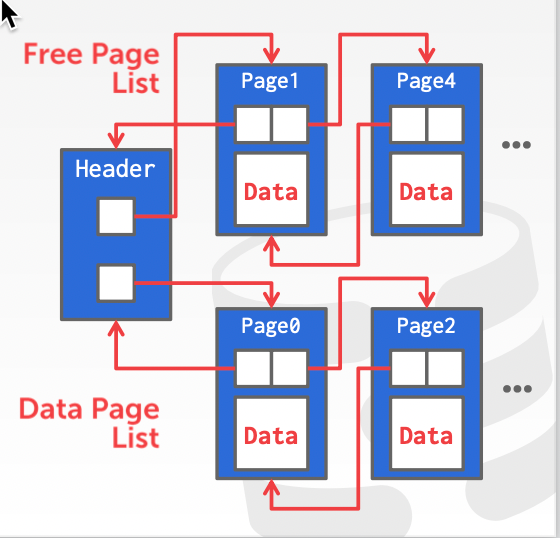
\includegraphics[width=.4\textwidth]{../images/15445/1.png}
\label{}
\end{figure}

The DBMS maintains special pages that tracks the location of data pages in the database files

The directory also records the number of free slots per page

must make sure that the directory pages are in sync with the data pages

\begin{figure}[htbp]
\centering
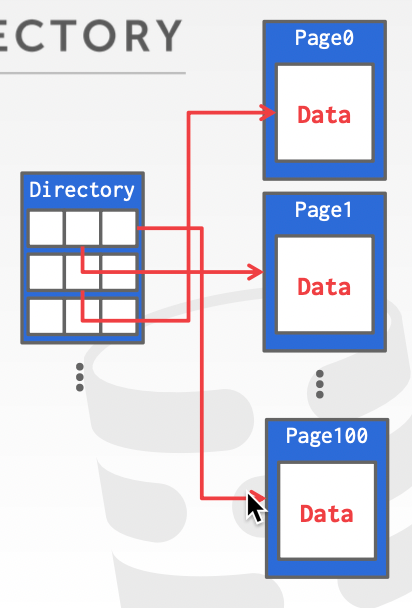
\includegraphics[width=.4\textwidth]{../images/15445/2.png}
\label{}
\end{figure}
\subsection{Page Layout}
\label{sec:org2835e29}
Every page contains a \textbf{header} of metadata about the page's content
\begin{itemize}
\item page size
\item checksum
\item DBMS version
\item transaction visibility
\item compression information
\end{itemize}
Some systems require pages to be self-contained

For any page storage architecture, we need to decide how to organize the data inside of the page

Two approaches
\begin{itemize}
\item tuple-oriented
\item log-structured
\end{itemize}

\textbf{Tuple-oriented}:

Strawman Idea: keep track of the number of tuples in a page and then just append a new tuple to
the end
\begin{itemize}
\item What happens if we delete a tuple
\item what happens if we have a variable-length attribute
\end{itemize}
\begin{figure}[htbp]
\centering
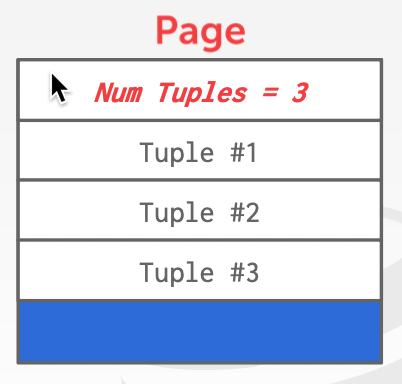
\includegraphics[width=.4\textwidth]{../images/15445/3.png}
\label{}
\end{figure}

The most common layout scheme is called \textbf{slotted pages}, the slot array maps ``slots'' to the
tuples' starting position offsets

The header keeps track of
\begin{itemize}
\item the \# of used slots
\item The offset of the starting location of the last slot used
\end{itemize}

\begin{figure}[htbp]
\centering
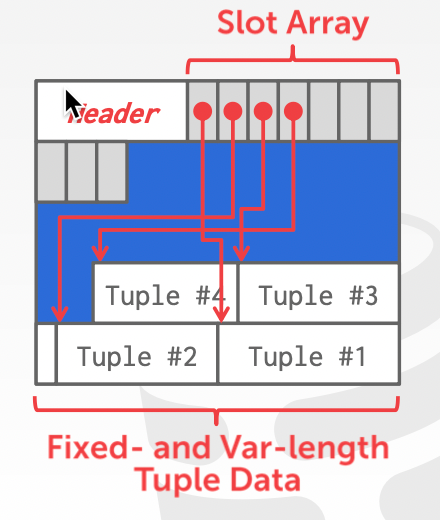
\includegraphics[width=.3\textwidth]{../images/15445/4.png}
\label{}
\end{figure}

The DBMS needs a way to keep track of individual tuples, each tuple is assigned a unique \textbf{record
identifier}
\begin{itemize}
\item most common: \texttt{page\_id} + \texttt{offset/slot}
\end{itemize}

An application cannot rely on these IDs to mean anything
\subsection{Tuple layout}
\label{sec:org524a9f8}
A tuple is essentially a sequence of bytes

It's the job of the DBMS to interpret those bytes into attribute types and values

Each tuple is prefixed with a \textbf{header} that contains meta-data about it
\begin{itemize}
\item visibility info
\item bit map for \texttt{NULL} values
\end{itemize}

We do \textbf{not} need to store meta-data about the schema

Attributes are typically stored in the order that you specify them when you create the table.

DBMS can physically \textbf{denormalize} (pre join) related tuples and store them together in the same
page
\begin{figure}[htbp]
\centering
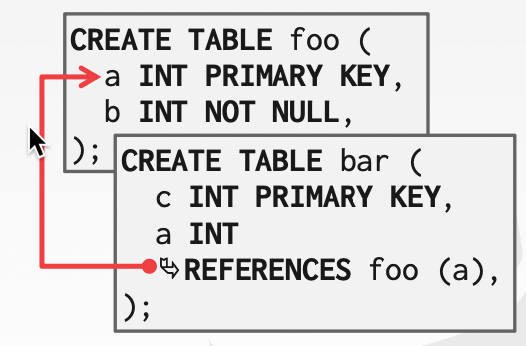
\includegraphics[width=.3\textwidth]{../images/15445/5.png}
\label{}
\end{figure}

\begin{figure}[htbp]
\centering
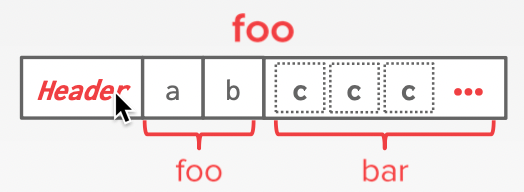
\includegraphics[width=.3\textwidth]{../images/15445/6.png}
\label{}
\end{figure}

Instead of storing tuples in pages, the DBMS only stores \textbf{log records}

The system appends log records to the file of how the database was modified
\begin{itemize}
\item inserts store the entire tuple
\item deletes mark the tuple as deleted
\item updates contain the delta of just the attributes that were modified
\end{itemize}

\begin{figure}[htbp]
\centering
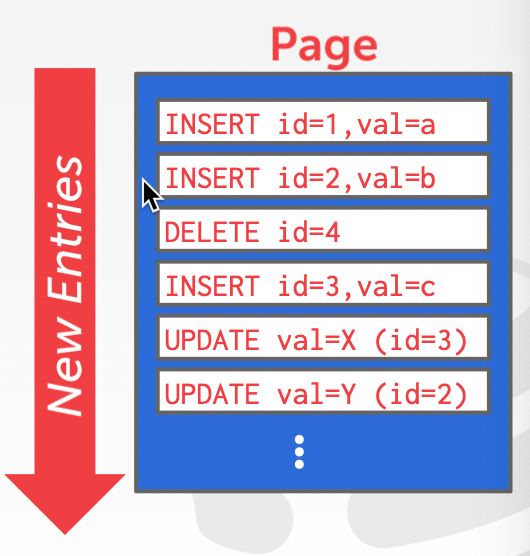
\includegraphics[width=.4\textwidth]{../images/15445/7.png}
\label{}
\end{figure}

To read as records, the DBMS scans the log backwards and ``recreates'' the tuple to find what it
needs

Build indexes to allow it to jump to locations in the log
\begin{figure}[htbp]
\centering
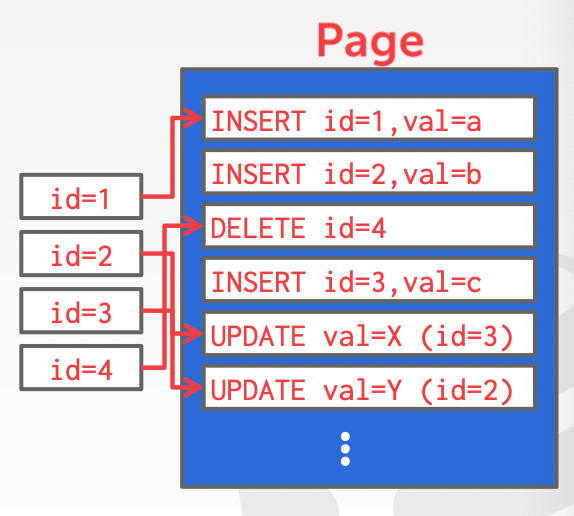
\includegraphics[width=.4\textwidth]{../images/15445/8.png}
\label{}
\end{figure}

Periodically compact the log
\begin{figure}[htbp]
\centering
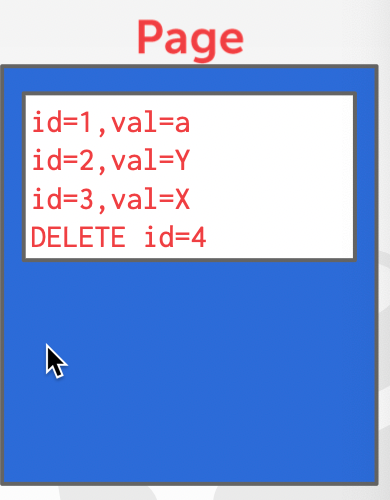
\includegraphics[width=.4\textwidth]{../images/15445/9.png}
\label{}
\end{figure}

Compaction coalesces larger log files into smaller files by removing unnecessary records
\begin{figure}[htbp]
\centering
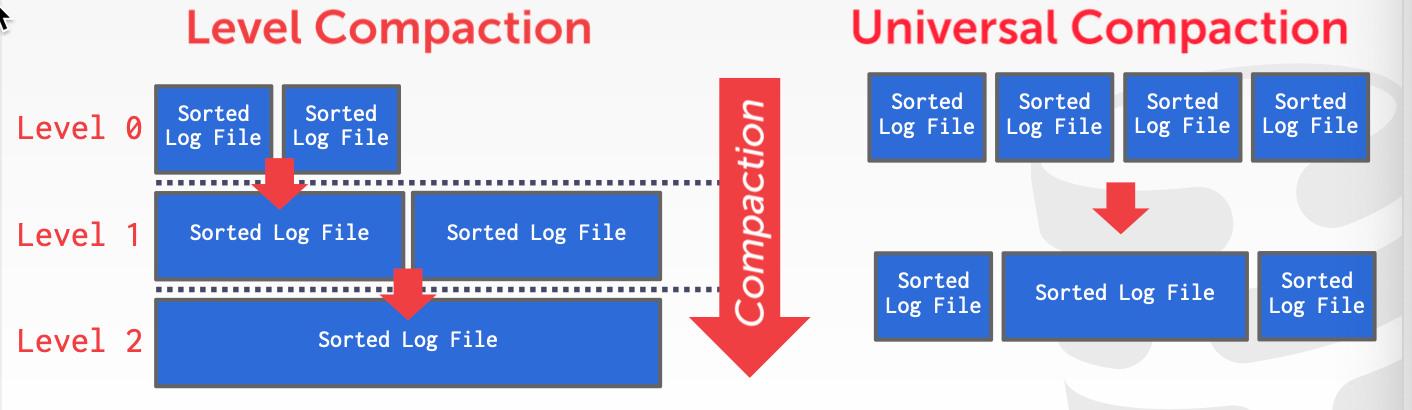
\includegraphics[width=.8\textwidth]{../images/15445/10.png}
\label{}
\end{figure}
\subsection{Data representation}
\label{sec:orga504da3}
\begin{itemize}
\item \texttt{INTEGER} / \texttt{BIGINT} / \texttt{SMALLINT} / \texttt{TINYINT}
C/C++ Representation
\item \texttt{FLOAT} / \texttt{REAL} vs. \texttt{NUMERIC} / \texttt{DECIMAL}

IEEE-754 Standard / Fixed-point Decimals

numerical/decimal is accurate without rounding errors
\item \texttt{VARCHAR} / \texttt{VARBINARY} / \texttt{TEXT} / \texttt{BLOB}

Header with length, followed by data bytes.
\item \texttt{TIME} / \texttt{DATE} / \texttt{TIMESTAMP}

32/64-bit integer of (micro)seconds since Unix epoch
\end{itemize}


To store values that are larger than a page, the DBMS uses separate \textbf{overflow} storage pages

\begin{figure}[htbp]
\centering
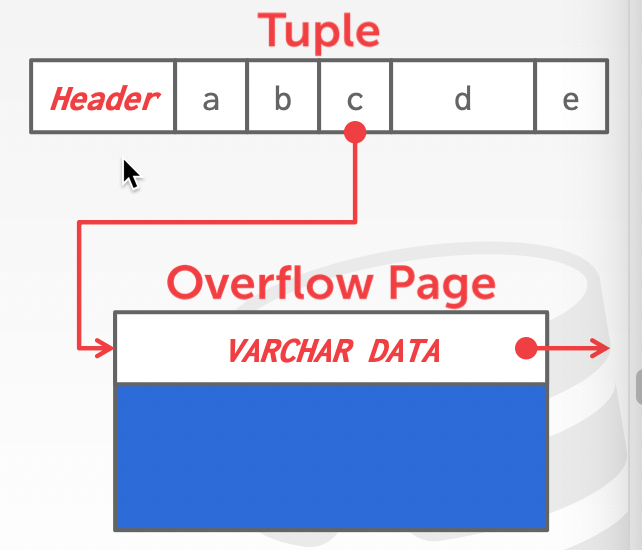
\includegraphics[width=.4\textwidth]{../images/15445/11.png}
\label{}
\end{figure}

Some systems allow you to store a really large value in an external file, treated as a \texttt{BLOB} type

The DBMS \textbf{cannot} manipulate the contents of an external file

\subsection{system catalogs}
\label{sec:org7e55cff}
A DBMS stores meta-data about databases in its internal catalogs
\begin{itemize}
\item tables, columns, indexes, views
\item users, permissions
\item internal statistics
\end{itemize}

Almost every DBMS stores the database's catalog inside itself

You can query the DBMS's internal \texttt{INFORMATION\_SCHEMA} catalog to get info about the database

\emph{List all the tables in the current database}:
\begin{minted}[]{sql}
/*SQL-92*/
SELECT *
FROM INFORMATION_SCHEMA.TABLES
WHERE table_catalog = '<db_name>';

/*Postgres*/
\d;

/*MySQL*/
SHOW TABLES;

/*SQLite*/
.tables
\end{minted}

\emph{List all the tables in the student table}
\begin{minted}[]{sql}
/*SQL-92*/
SELECT *
FROM INFORMATION_SCHEMA.TABLES
WHERE table_catalog = 'student';

/*Postgres*/
\dstudent;

/*MySQL*/
DESCRIBE student;

/*SQLite*/
.schema student
\end{minted}

Database workloads:
\begin{itemize}
\item On-line transaction processing (OLTP)

fast operations that only read/update a small amount of data each time
\item On-line analytical processing (OLAP)

complex queries that read a lot of data to compute aggregates
\item Hybrid transaction + analytical processing (HTAP)

OLTP+OLAP together on the same database instancew
\end{itemize}
\subsection{storage models}
\label{sec:orgffea034}
The DBMS cna store tuples in different ways that are better for either OLTP or OLAP workloads

We haven been assuming the \(n\)-ary storage model so fart this semester

\textbf{n-ary storage model (NSM)}: the DBMS stores all attributes for a single tuple contiguously in a
 page

Ideal for OLTP workloads where queries tend to operate only on an individual entity and
insert-heavy workloads

\begin{figure}[htbp]
\centering
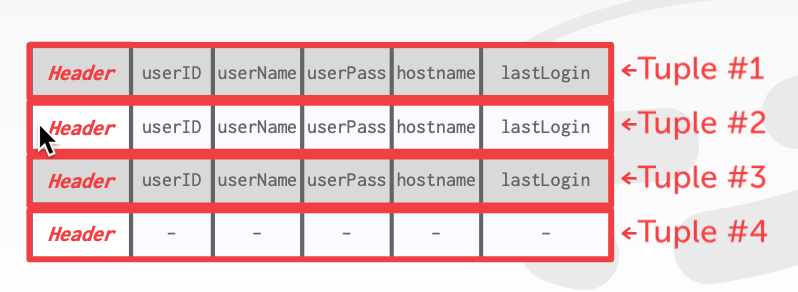
\includegraphics[width=.5\textwidth]{../images/15445/12.png}
\label{}
\end{figure}

\begin{figure}[htbp]
\centering
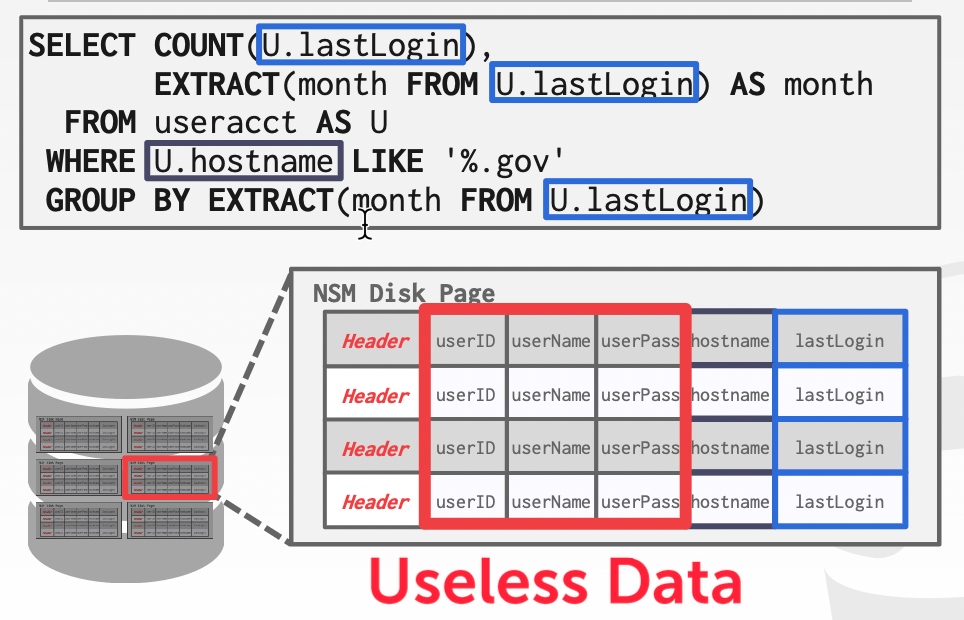
\includegraphics[width=.5\textwidth]{../images/15445/13.png}
\label{}
\end{figure}

Advantages
\begin{itemize}
\item fast insertions, updates and deletes
\item Good for querries that need the entire tuple
\end{itemize}
Disadvantages
\begin{itemize}
\item not good for scanning large portions of the table and/or a subset of the attributes
\end{itemize}

\textbf{decomposition storage model (DSM)}: the DBMS stores the values of a single attribute for all
 tupoles contiguously in a page
\begin{itemize}
\item also known as a ``column store''
\end{itemize}
\begin{figure}[htbp]
\centering
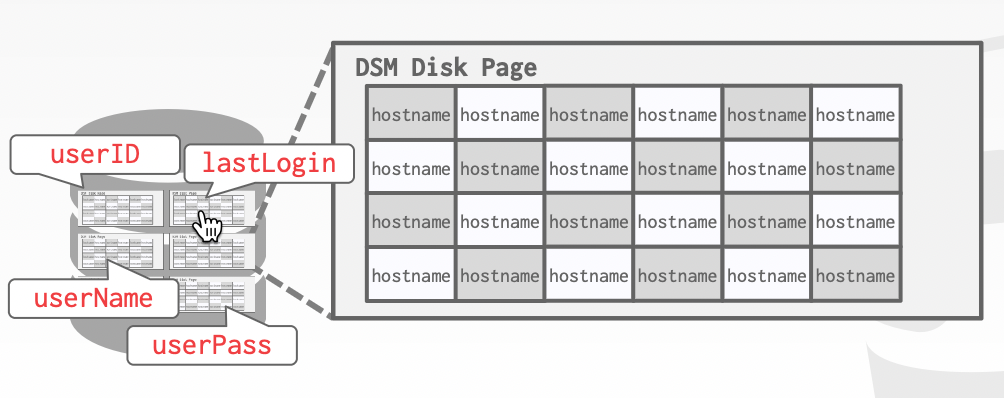
\includegraphics[width=.5\textwidth]{../images/15445/14.png}
\label{}
\end{figure}

Tuple identification:
\begin{itemize}
\item fixed-length offsets

each value is the same length for an atrribute
\item embedded tuple Ids

each value is stored with its tuple id in a column
\end{itemize}
\section{Buffer Pools}
\label{sec:orga1c79e8}
How the DBMS manages its memory and move data back-and-forth from disk

\begin{itemize}
\item spatial control
\begin{itemize}
\item where to write pages on disk
\item the goal is to keep pages that are used together often as physically close together as
possible on disk
\end{itemize}
\item temporal control
\begin{itemize}
\item when to read pages into memory, and when to write them to disk
\item the goal is to minimize the number of stalls from having to read data from disk
\end{itemize}
\end{itemize}
\subsection{Buffer Pool Manager}
\label{sec:org1284901}
Memory region organized as an array of fixed-size pages. An array entry is called a \textbf{frame}

When  the DBMS requests a page, an exact copy is places into one of these frames

The \textbf{page table} keeps track of pages that are currently in memory

Also maintains additional meta-data per page
\begin{itemize}
\item dirty flag
\item pin/reference counter
\end{itemize}

\textbf{Locks}
\begin{itemize}
\item protects the database's logical contents from other transactions
\item held for transaction duration
\item need to be able to rollback changes
\end{itemize}

\textbf{Latches}
\begin{itemize}
\item protects the critical sections of the DBMS's internal data structure from other threads
\item held for operation duration
\item do not need to be able to rollback changes
\end{itemize}

The \textbf{page directory} is the mapping from page ids to page locations in the database files
\begin{itemize}
\item all changes must be recorded on disk to allow the DBMS to find on restart
\end{itemize}

The \textbf{page table} is the mapping from page ids to a copy of the page in buffer pool frames
\begin{itemize}
\item this is an in-memory data structure that does not need to be stored on disk
\end{itemize}

Buffer pool optimizations
\begin{itemize}
\item multiple buffer pools
\item pre-fetching
\item scan sharing
\item buffer pool bypass
\end{itemize}
\subsubsection{Multiple Buffer Pools}
\label{sec:org472e606}
The DBMS does not always have a single buffer pool for the entire system
\begin{itemize}
\item multiple buffer pool instances
\item per-database buffer pool
\item per-page type buffer pool
\end{itemize}

Helps reduce latch contention and improve locality

Approach 1: Object Id
\begin{itemize}
\item Embed an object identifier in record ids and then maintain a mapping from objects to specific
buffer pools
\end{itemize}

Approach 2: Hashing
\begin{itemize}
\item Hash the page id to select which buffer pool to access
\end{itemize}
\subsubsection{Pre-fetching}
\label{sec:orgd5389d9}
The DBMS can also prefetch pages based on query plan
\subsubsection{Scan Sharing}
\label{sec:org1f61414}
Queries can reuse data retrieved from storage or operator computations
\begin{itemize}
\item Also called \textbf{synchronized scans}
\end{itemize}

Allow multiple queries to attach to a single cursor that scans a table
\begin{itemize}
\item queries don't have to be the same
\item can also share intermediate results
\end{itemize}
\subsubsection{Buffer Pool Bypass}
\label{sec:orgb731d9d}
The sequential scan operator won't store fetched pages in the buffer pool to avoid overhead
\subsection{Replacement Policies}
\label{sec:orgf7d48a0}
Least-recently  used

Approximation of LRU that does not need a separate timestamp per page
\begin{itemize}
\item each page has a reference bit
\item when a page is accessed, set to 1
\end{itemize}

Organize the pages in a circular buffer with a clock hand
\begin{itemize}
\item upon sweeping, check if a page's bit is set to 1
\item if yes, set to zero. If no, then evict
\end{itemize}

Better policies:
\begin{itemize}
\item LRU-K

Track the history of last K references to each page as timestamps and compute the interval
between subsequent accesses

The DBMS then uses this history to estimate the next time that page is going to be accessed
\item The DBMS chooses which pages to evict on a per txn/query basis.
\end{itemize}


\subsection{Other Memory Pools}
\label{sec:org2204dac}
\begin{itemize}
\item sorting + join buffers
\item query caches
\item maintenance buffers
\item log buffers
\item dictionary caches
\end{itemize}
\section{Hashtables}
\label{sec:org4b96fde}
We are now going to talk about how to support the DBMS's execution engine to read/write data
from pages

\subsection{Hash functions}
\label{sec:org93967e8}
\begin{itemize}
\item crc-64 (1975)
\item murmurhash (2008)
\item google cityhash (2011)
\item facebook xxhash (2012)
\item google farmhash (2014)
\end{itemize}

\subsection{static hashing schemes}
\label{sec:org71a2077}
\subsubsection{linear probe hashing}
\label{sec:org0f07d56}
single giant table of slots

resolve collisions by linearly searching for the next free slot in the table
\begin{itemize}
\item to determine whether an element is present, hash to a location in the index and scan for it
\item must store the key in the index to know when to stop scanning
\item insertions and deletions are generalizations of lookups
\end{itemize}

delete: support A and B are hashed into the same location and then B is the next element of A,
now if we delete A, how do we find the B
\begin{itemize}
\item tombstone
\item movement
\end{itemize}

For non-unique keys,
\begin{enumerate}
\item separated linked list
\item redundant keys
\end{enumerate}

\begin{figure}[htbp]
\centering
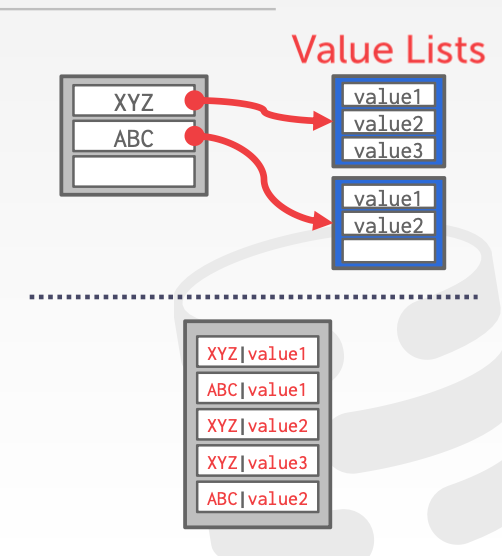
\includegraphics[width=.4\textwidth]{../images/15445/15.png}
\label{}
\end{figure}
\subsubsection{robin hood hashing}
\label{sec:orgd2dc47f}
Variant of linear probe hashing that steals slots from ``rich'' keys and give them to ``poor'' keys.
\begin{itemize}
\item Each key tracks the number of positions they are from where its optimal position in the table.
\item On insert, a key takes the slot of another key if the first key is farther away from its
optimal position than the second key.
\end{itemize}
\subsubsection{cuckoo hashing}
\label{sec:orga8b2fbf}
Use multiple hash tables with different hash functions seeds
\begin{itemize}
\item on insert, check every table and pick anyone that has a free slot
\item if no table has a free slot, evict the element from one of them and then re-hash it find a new
location
\end{itemize}
Look-ups and deletions are always O(1) because only one location per hash table is checked
\subsection{dynamic hashing schemes}
\label{sec:org25cf221}
\subsubsection{Chained hashing}
\label{sec:orga5cfb00}
maintain a linked list of \textbf{buckets} for each slot in the hash table

resolve collisions by replacing all elements with the same hash key into the same bucket
\begin{itemize}
\item to determine whether an element is present, hash to its buckets and scan for it
\end{itemize}
\begin{figure}[htbp]
\centering
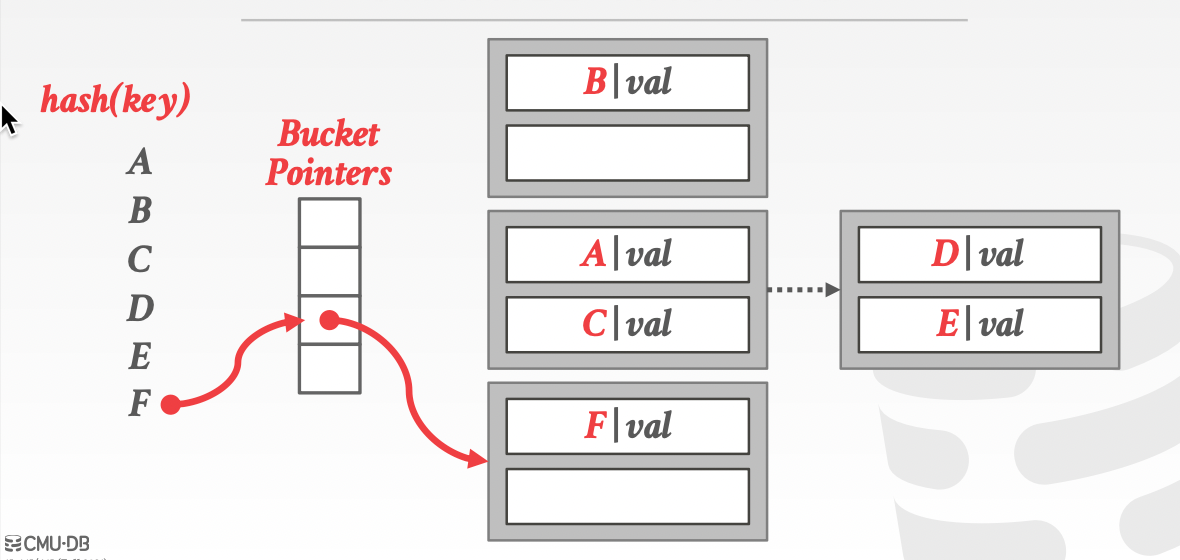
\includegraphics[width=.6\textwidth]{../images/15445/16.png}
\label{}
\end{figure}
\subsubsection{extendible hashing}
\label{sec:orgd037951}
\href{https://emunix.emich.edu/\~shaynes/Papers/ExtendibleHashing/extendibleHashing.html}{better source}

chained-hashing approach where we split buckets instead of letting the linked list grow forever

multiple slot locations can point to the same bucket chain

reshuffle bucket entires on split and increase the number of bits to examine

\begin{figure}[htbp]
\centering
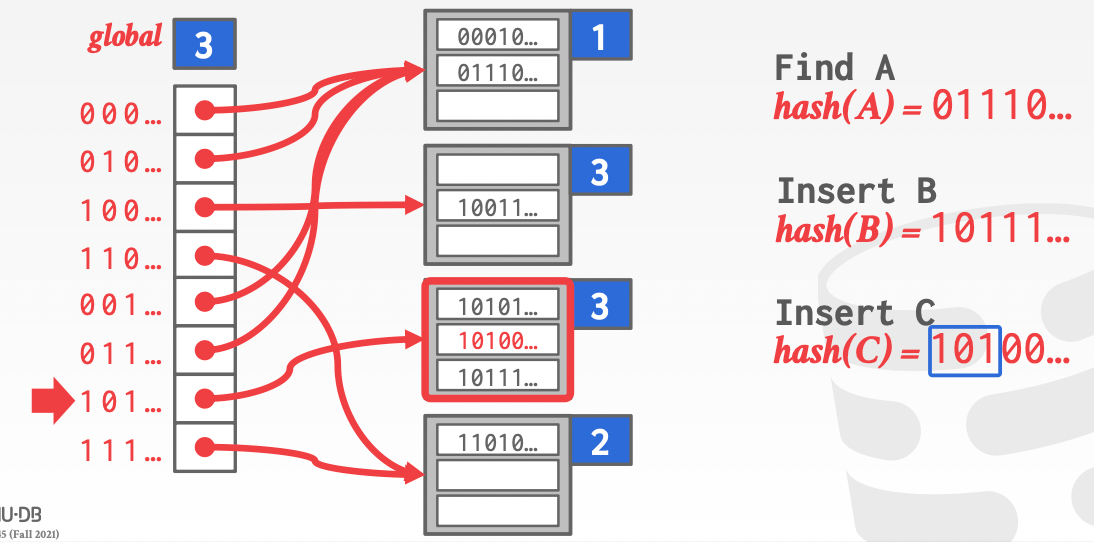
\includegraphics[width=.6\textwidth]{../images/15445/17.png}
\label{}
\end{figure}
\subsubsection{linear hashing}
\label{sec:orgbf7068a}
The hash table maintains a \textbf{pointer} that tracks the next bucket to split
\begin{itemize}
\item when any bucket overflows, split the bucket at the pointer location
\end{itemize}

use multiple hashes to find the right bucket for a given key

can use different overflow criterion
\section{Tree Indexes}
\label{sec:org49b4755}
A \textbf{table index} is a replica of a subset of a table's attributes that are organized and/or sorted
for efficient using those attributes
\subsection{B+ Tree overview}
\label{sec:orga9f4faf}
B-tree, B+tree, B*tree, Blink-tree

A B+Tree is a self-balancing tree data structure that keeps data sorted and allows searches,
sequential access, insertions and deletions in \(O(\log n)\)
\begin{itemize}
\item optimized for systems that read and write large blocks of data
\end{itemize}

A B+Tree is an \(M\)-way search tree with the following properties
\begin{itemize}
\item it is perfectly balanced (i.e., every leaf node is at the same depth in the tree)
\item every node other than the root is at least half-full \(M/2-1\le\text{\#keys}\le M-1\)
\item every inner node with \(k\)  keys has \(k+1\) non-null children
\end{itemize}
\begin{figure}[htbp]
\centering
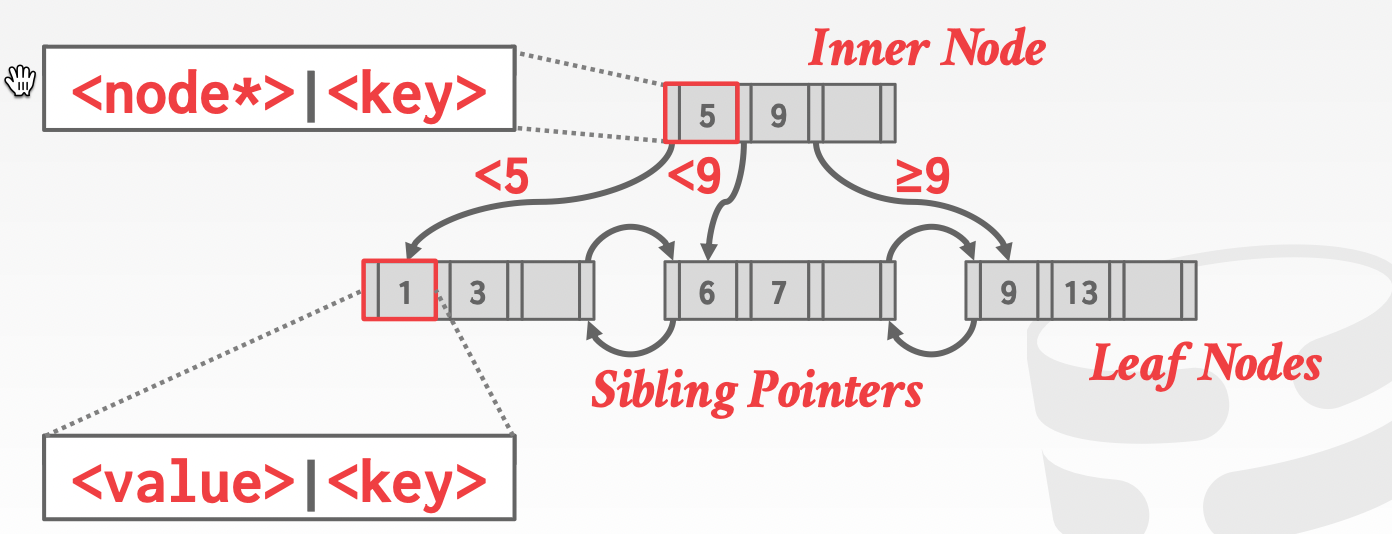
\includegraphics[width=.7\textwidth]{../images/15445/18.png}
\label{}
\end{figure}

Every B+Tree node is comprised of an array of key/value pairs
\begin{itemize}
\item the keys are derived from  the attributes that the index is based on
\item the values will differ based on whether the node is classified as an \textbf{inner node} or a \textbf{leaf node}
\end{itemize}

The arrays are (usually) kept in sorted key order

Leaf node values approach
\begin{enumerate}
\item record IDs

A pointer to the location of the tuple to which the index corresponds

\item tuple data

the leaf nodes store the actual contents of the tuple

secondary indexes must store the record ID as their values
\end{enumerate}

\textbf{Insert}
\begin{enumerate}
\item find correct leaf node L
\item put data entry into L in sorted order
\item if L has enough space, done
\item otherwise, split L keys into L and a new node L2
\begin{itemize}
\item redistribute entries evenly, copy up middle key
\item insert index entry pointing to L2 into parent of L
\end{itemize}
\end{enumerate}

\textbf{Delete}
\begin{enumerate}
\item find leaf L where entry belongs. remove the entry
\item if L is at least half-full, done
\item if L has only M/2-1 entries
\begin{itemize}
\item try to re-distribute, borrowing from sibling
\item if re-distribution fails, merge L and sibling
\end{itemize}
\end{enumerate}
If merge occured, must delete entry from parent of L

\textbf{Duplicate keys}
\begin{enumerate}
\item append record ID
\begin{itemize}
\item add the tuple's unique record ID as part of the key to ensure that all keys are unique
\item the DBMS can still use partial keys to find the tuples
\end{itemize}
\item Overflow leaf nodes
\begin{itemize}
\item allow leaf nodes to spill into overflow nodes that contain the duplicate keys
\end{itemize}
\end{enumerate}

\textbf{clustered indexes}
The table is stored in the sort order specified by the primary key
\begin{itemize}
\item can be either heap- or index-organized storage
\end{itemize}

some DBMS always use a clustered index
\begin{itemize}
\item if a table does not contain a primary key, the DBMS will automaticall y make a hidden primary key
\end{itemize}
\subsection{use in a DBMS}
\label{sec:orgfe4f2fa}
\subsection{Design choices}
\label{sec:org76b1951}
\subsubsection{node size}
\label{sec:org85c005a}
the slower the storage device, the larger the optimal node size for a B+ Tree
\begin{itemize}
\item HDD: 1MB
\item SSD: 10KB
\item In-Memory: 512B
\end{itemize}

optimal sizes can vary depending on the workload


\subsubsection{merge threshold}
\label{sec:org74b7b2d}
some DBMSs do not always merge nodes when they are half full

delaying a merge operation may reduce the amount of reorganization

it may also be better to just let smaller nodes exist and then periodically rebuild entire tree

\subsubsection{variable-length keys}
\label{sec:orgf8dada3}
\begin{enumerate}
\item pointers
\item variable-length nodes
\item padding
\item key map / indirection
\end{enumerate}
\subsubsection{intra-node search}
\label{sec:org5dc3803}
\begin{enumerate}
\item linear
\item binary
\item interpolation
\end{enumerate}
\subsection{optimizations}
\label{sec:org2d7c17f}
\subsubsection{prefix compression}
\label{sec:org0613cfd}
sorted keys in the smae leaf node are likely to have the same prefix
\begin{center}
\begin{tabular}{lll}
robbed & robbing & robot\\
\end{tabular}
\end{center}

Instead of storing the entire key each time, extract common prefix and store only unique suffix
for each key
\subsubsection{deduplication}
\label{sec:orga50eb30}
non-unique indexes can end up storing multiple copies of the same key in leaf nodes

the leaf node can store the key once and then maintain a list of tuples with that key
\subsubsection{bulk insert}
\label{sec:org735ea04}
The fastest way to build a new B+Tree for an existing table is to first sort the keys and then
rebuild the index from the bottom up
\section{Index Concurrency}
\label{sec:org869275e}
\subsection{Latches Overview}
\label{sec:org6b51bd3}
\textbf{Locks}
\begin{itemize}
\item protect the database's logical contents from other txns
\item held for txn duration
\item need to be able to rollback changes
\end{itemize}

\textbf{Latches}
\begin{itemize}
\item Protect the critical sections of the DBMS's internal data structure from other threads
\item held for operation duration
\item do not need to be able to rollback changes
\end{itemize}

\begin{center}
\begin{tabular}{lll}
 & Locks & Latches\\
Separate & User Txns & Threads\\
Protect & Database Contents & In-Memory Data Structures\\
During & Entire Txns & Critical Sections\\
Modes & Shared, Exclusive, Update, Intention & Read, Write\\
Deadlock & Detection \& Resolution & Avoidance\\
by & Waits-for, Timeout, Aborts & Coding Discipline\\
Kept in & Lock Manager & Protected Data Structure\\
\end{tabular}
\end{center}

\subsubsection{Latch Modes}
\label{sec:orgc533933}
\textbf{Read Mode}
\begin{itemize}
\item Multiple threads can read the same object at the same time
\item A thread can acquire the read latch if another thread has it in read mode
\end{itemize}

\textbf{Write Mode}
\begin{itemize}
\item Only one thread an access the object
\item A thread cannot acquire a write latch if another thread has it in any mode
\end{itemize}

\subsubsection{Latch Implementations}
\label{sec:org88b1284}
\begin{enumerate}
\item Blocking OS Mutex
\label{sec:org9a3d496}
non-scalable (about 25ns per lock/unlock invocation)

\begin{minted}[]{c++}
std::mutex m;

m.lock();

m.unlock();
\end{minted}

But \texttt{std::mutex} -> \texttt{pthread\_mutex\_t} -> \texttt{futex}
\item Test-and-Set Spin Latch (TAS)
\label{sec:org1c9c828}
\begin{itemize}
\item very efficient (single instruction to latch/unlatch)
\item non-scalable, not cache-friendly, not OS-friendly
\item \texttt{std::atomic<T>}
\end{itemize}

\begin{minted}[]{c++}
std::atomic_flag latch;

while (latch.test_and_set(...)) {

}
\end{minted}

\textbf{Do not use spinlocks in user space, unless you actually know what you're doing}. And be aware
that the likelihood that you know what you are doing is basically nil.
\item Read-Writer Latches
\label{sec:org917896b}
\begin{itemize}
\item Allows for concurrent readers
\item Must manage read/write queues to avoid starvation
\item can be implemented on top of spin latches
\end{itemize}
\end{enumerate}

\subsection{Hash table latching}
\label{sec:orgf4a5d50}
easy to support concurrent access due to the limited ways threads access the data structure
\begin{itemize}
\item all threads move in the same direction and only access a single page/slot at a time
\item deadlocks are not possible
\end{itemize}

To resize the table, take a global write latch on the entire table

\begin{enumerate}
\item Page latches
\begin{itemize}
\item each page has its own reader-writer latch that protects its entire contents
\item threads acquire either a read or write latch before they access a page
\end{itemize}
\item Slot latches
\begin{itemize}
\item each slot has its own latch
\item can use a single-mode latch to reduce meta-data and computational overhead
\end{itemize}
\end{enumerate}

Atomic instruction that compares contents of a memory location M to a given value V
\texttt{\_\_sync\_bool\_compare\_and\_swap(\&M,20,30)}
\begin{itemize}
\item if values are equal, installs new given value V' in M
\item otherwise operation fails
\end{itemize}

\subsection{B+Tree Latching}
\label{sec:org9684cae}
We want to allow multiple threads to read and update a B+ Tree at the same time

We need to protect against two types of problems
\begin{itemize}
\item threads trying to modify the contents of a node at the same time
\item one thread traversing the tree while another thread splits/merge nodes
\end{itemize}
\subsubsection{Latch crabbing/coupling}
\label{sec:orga22df85}
Protocol to allow multiple threads to access/modify B+ Tree at the same time

\textbf{Basic idea}:
\begin{itemize}
\item get latch for parent
\item get latch for child
\item release latch for parent if ``safe''
\end{itemize}

A \textbf{safe node} is one that will not split or merge when updated
\begin{itemize}
\item not full
\item more than half-full
\end{itemize}

\textbf{Find}: start at root and go down
\begin{itemize}
\item acquire R latch on child
\item then unlatch parent
\end{itemize}

\textbf{Insert/Delete}: Start at root and go down, obtaining W latches as needed. Once child is latched,
 check if it is safe:
\begin{itemize}
\item if child is safe, release all latches on ancestors
\end{itemize}

But taking a write latch on the root every time becomes a bottleneck with higher concurrency
\subsubsection{Better latching algorithm}
\label{sec:orgf411dd2}
Most modifications to a B+Tree will \uline{not} require a split or merge

Instead of assuming that there will be a split/merge, optimistically traverse the tree using
read latches

If you guess wrong, repeat traversal with the pessimistic algorithm

\textbf{Search}: same as before

\textbf{Insert/Delete}:
\begin{itemize}
\item set latches as if for search, get to leaf, and set W latch on leaf
\item if leaf is not safe, release all latches, and restart thread using previous insert/delete
protocol with write latches
\end{itemize}

This approach optimistically assumes that only leaf node will be modified; if not, R latches set
on the first pass to leaf are wasteful
\subsection{Leaf Node Scans}
\label{sec:org349e9c6}
The threads in all the examples so far have acquired latches in a ``top-down'' manner

But what if we want to move from one leaf node to another leaf node?

Latches do not support deadlock detection or avoidance. The only way we can deal with this
problem is through coding discipline

The leaf node sibling latch acquisition protocol must support a ``no-wait'' mode

The DBMS's data structures must cope with failed latch acquisitions
\section{Sorting \& Aggregations}
\label{sec:org7ec851f}
\subsection{External Mergre Sort}
\label{sec:org81436b2}
What do we need to sort
\begin{itemize}
\item relational model/SQL is unsorted
\item queries may request that tuples are sorted in a specific way
\item But even if a query does not specify an order, we may still want to sort to do other things
\begin{itemize}
\item trivial to support duplicate elimination
\item bulk loading sorted tuples into a B+ tree index is faster
\item aggregations
\end{itemize}
\end{itemize}
\subsubsection{2-way external merge sort}
\label{sec:org0b7b0ec}
2 is the number of runs that we are going to merge into a new run for each pass

data is broken up into N pages

the DBMS has a finite number of B buffer pool pages to hold input and output data

\textbf{Pass 0}
\begin{itemize}
\item read all B pages of the table into memory
\item sort pages into runs and write them back to disk
\end{itemize}

\textbf{Pass 1,2,3,..}
\begin{itemize}
\item recursively merge pairs of runs into runs twice as long
\item uses three buffer pages (2 for input pages, 1 for output)
\end{itemize}

Number of pass: \(1+\lceil\log_2N\rceil\)

Total I/O cost: \(2N\cdot(\#\text{ of passes})\)

\begin{figure}[htbp]
\centering
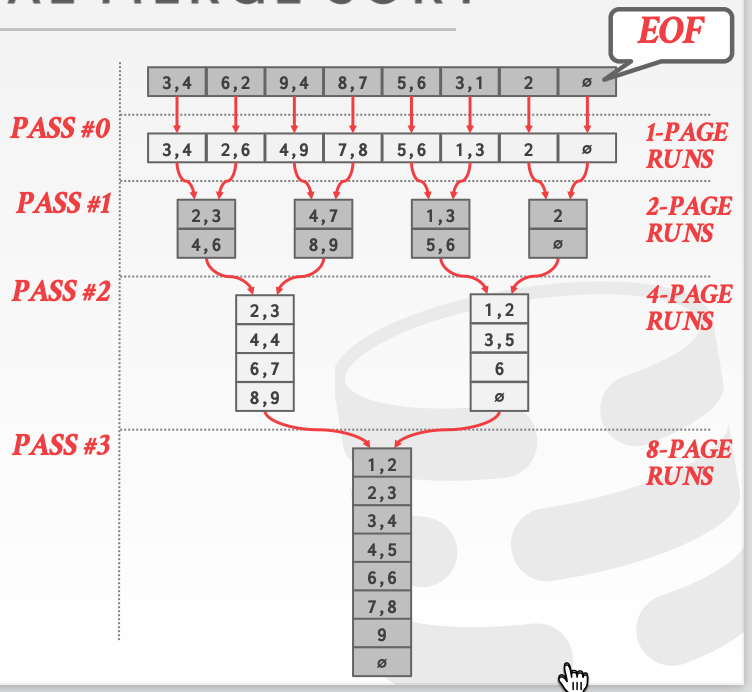
\includegraphics[width=.6\textwidth]{../images/15445/19.png}
\label{}
\end{figure}

This algorithm only requires three buffer pool pages to perform the sorting

\textbf{Double buffering optimization}
Prefetch the next run in the background and store it in a second buffer while system is
processing the current run
\begin{itemize}
\item reduces the wait time for I/O requests at each step
\end{itemize}
\subsubsection{General external merge sort}
\label{sec:org77e021d}
\textbf{Pass 0}
\begin{itemize}
\item use B buffer pages
\item produce \(\lceil N/B\rceil\) sorted runs of size B
\end{itemize}

\textbf{Pass 1}
\begin{itemize}
\item merge \(B-1\) runs
\end{itemize}

Number of pass: \(1+\lceil\log_{B-1}\lceil N/B\rceil\rceil\)

Total I/O cost: \(2N\cdot(\#\text{ of passes})\)
\subsubsection{Using B+Trees for sorting}
\label{sec:org7b4f256}

\subsection{Aggregations}
\label{sec:orgb7bf67e}
Two implementation choices
\begin{itemize}
\item sorting
\item hashing
\end{itemize}

\begin{figure}[htbp]
\centering
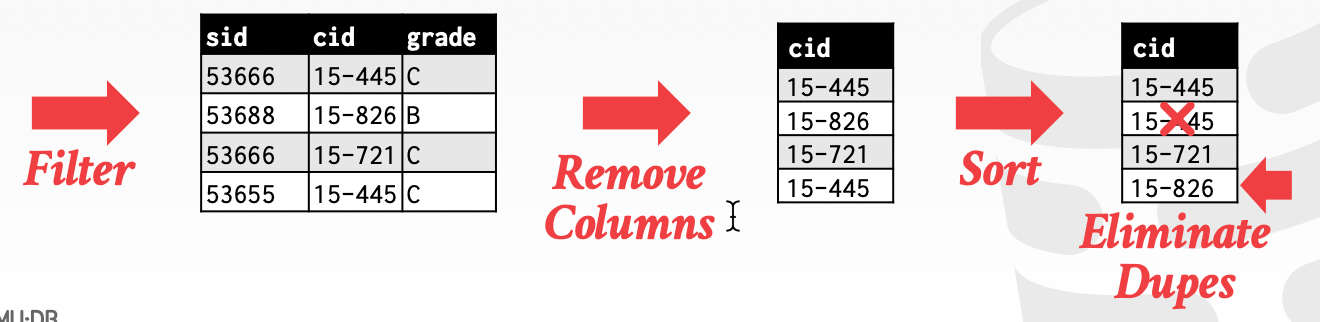
\includegraphics[width=.8\textwidth]{../images/15445/20.png}
\label{}
\end{figure}

\textbf{Hashing aggregate}: Populate an ephemeral hash table as the DBMS scans the table. For each
 record, check whether there is already an entry in the hash table:
\begin{itemize}
\item \texttt{DISTINCT}: discard duplicate
\item \texttt{GROUP BY}: perform aggregate computation
\end{itemize}

If everything fits in memory, then this is easy


\subsubsection{External hashing aggregate}
\label{sec:org66a6043}
\begin{enumerate}
\item Phase 1: Partition
\label{sec:org2b39217}
\begin{itemize}
\item divide tuples into buckets based on hash key
\item write them out to disk when they get full
\end{itemize}

use a hash function \(h_1\) to split tuples into \textbf{partitions} on disk
\begin{itemize}
\item a partition is one or more pages that contain the set of keys with the same hash value
\item partitions are ``spilled'' to disk via output buffers
\end{itemize}

Assume that we have B buffers, we will use B-1 buffers for the partitions and 1 buffer for the
input data

\begin{figure}[htbp]
\centering
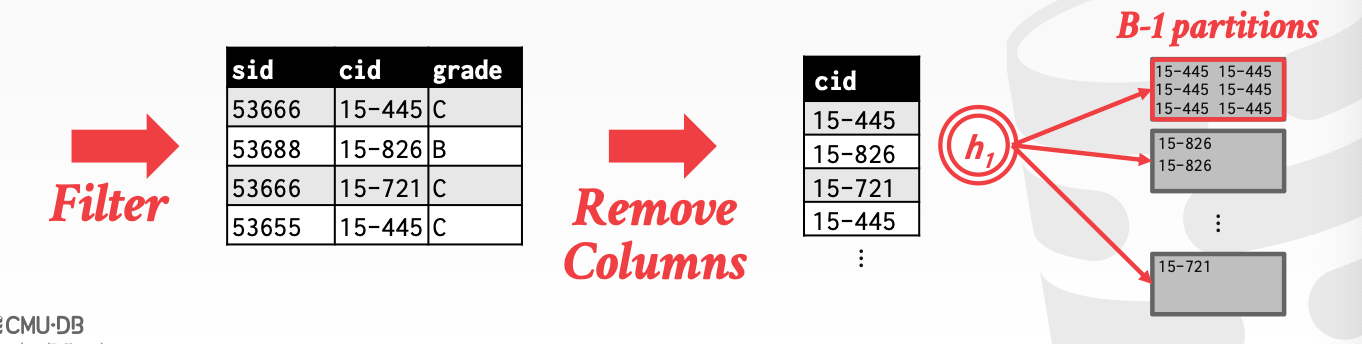
\includegraphics[width=.8\textwidth]{../images/15445/21.png}
\label{}
\end{figure}

\item Phase 2: ReHash
\label{sec:org14e7255}
\begin{itemize}
\item build in-memory hash table for each partition and compute the aggregation
\end{itemize}

For each partition on disk
\begin{itemize}
\item read it into memory and build an in-memory hash table based on a second hash function \(h_2\)
\item then go through each bucket of this hash table to bring together matching tuples
\end{itemize}

This assumes that each partition fits in memory
\end{enumerate}

\subsubsection{Hashing summarization}
\label{sec:org886a76d}
During the rehash phase, store pairs of the form \texttt{GroupKey->RunningVal}

when we want to insert a new tuple into the hash table
\begin{itemize}
\item if we find a matching \texttt{GroupKey}, just update the \texttt{RunningVal} appropriately
\item else insert a new \texttt{GroupKey->RunningVal}
\end{itemize}

\begin{figure}[htbp]
\centering
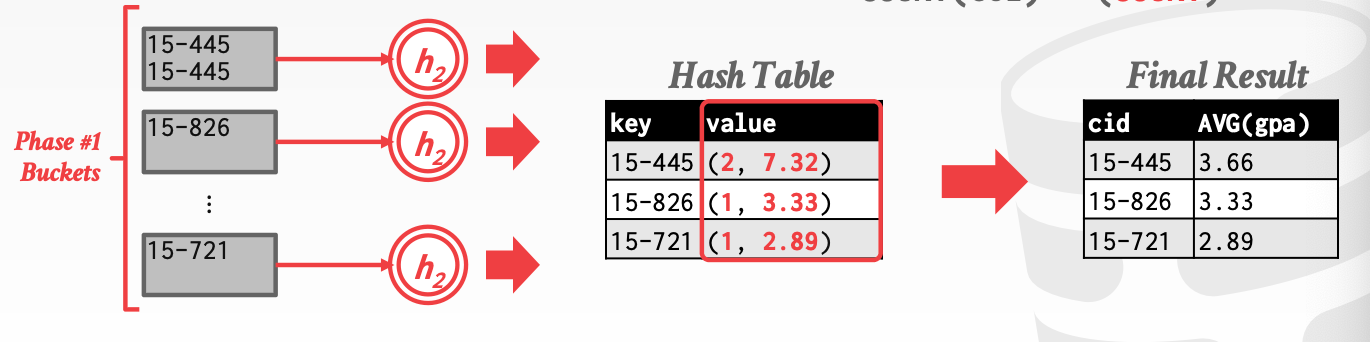
\includegraphics[width=.8\textwidth]{../images/15445/22.png}
\label{}
\end{figure}


\section{Joins}
\label{sec:org136b96d}
We will focus on performing binary joins (two tables) using \textbf{inner equijoin} algorithms
\begin{itemize}
\item these algorithms can be tweaked to support other joins
\item multi-way joins exist primarily in research literature
\end{itemize}

In general, we want the smaller table to always be the left table (``outer table'') in the query
plan

\textbf{Decision 1}: output
\begin{itemize}
\item what data does the join operator emit to its parent operator in the query plan tree
\end{itemize}

\textbf{Decision 2}: cost analysis criteria
\begin{itemize}
\item how do we determine whether one join algorithm is better than another
\end{itemize}

\begin{minted}[]{sql}
SELECT R.id, S.cdate
  FROM R JOIN S
    ON R.id = S.id
 WHERE S.value > 100
\end{minted}

\begin{figure}[htbp]
\centering
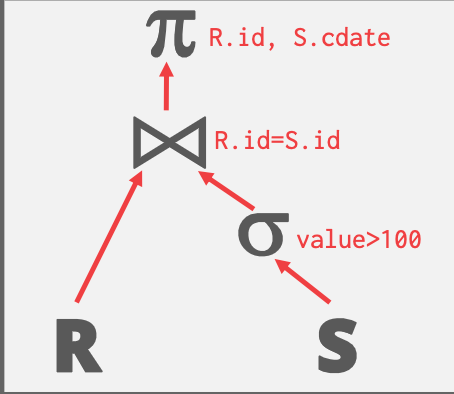
\includegraphics[width=.3\textwidth]{../images/15445/23.png}
\label{}
\end{figure}

For tuple \(r\in R\) and tuple \(s\in S\) that match on join attributes, concatenate \(r\) and \(s\)
together into a new tuple

output contents can vary:
\begin{itemize}
\item depends on processing model
\item depends on storage model
\item depends on data requirements in query
\end{itemize}

\textbf{Early Materialization}:
\begin{itemize}
\item copy the values for the attributes in outer and inner tuples into a new output tuple
\item subsequent operators in the query plan never need to go back to the base tables to get more
data
\end{itemize}

\textbf{Late Materialization}:
\begin{itemize}
\item only copy the joins keys along with the Record IDs of the matching tuples
\item ideal for column stores because the DBMS does not copy data that is not needed for the query
\end{itemize}

\textbf{Cost Analysis Criteria}

Assume
\begin{itemize}
\item \(M\) pages in table \(R\), \(m\) tuples in \(R\)
\item \(N\) pages in table \(S\), \(n\) tuples in \(S\)
\end{itemize}

\textbf{Cost Metric}: \# of IOs to compute join

\(R\bowtie S\) is the most common operation and thus must be carefully optimized

\(R\times S\) followed by a selection is inefficient because the cross-product is large

\subsection{Join algorithms}
\label{sec:org79deb8c}

\subsubsection{Nested Loop Join}
\label{sec:org503d4f5}
\begin{enumerate}
\item Simple/Stupid
\label{sec:orge6a68a8}
foreach tuple \(r\in R\):
    foreach tuple \(s\in S\):
        emit, if \(r\) and \(s\) match

Cost: \(M+m\cdot N\)
\item Block
\label{sec:org3daec31}
foreach block \(B_R\in R\)
    foreach block \(B_S\in S\)
        foreach tuple \(r\in B_r\)
            foreach tuple \(s\in B_s\)
                emit, if \(r\) and \(s\) match

cost: \(M+M\cdot N\)

What if we have B buffers available?
\begin{itemize}
\item use \(B-2\) buffers for scanning the outer table
\item use one buffer for the inner table, one buffer for storing output
\end{itemize}

foreach \(B-2\) blocks \(b_R\in R\)
    foreach block \(b_S\in S\)
        foreach tuple \(r\in B-2\) blocks
            foreach tuple \(s\in b_S\)
                emit, if \(r\) and \(s\) match

Cost: \(M+\lceil M/(B-2)\rceil\cdot N\)
\item Index
\label{sec:org2957c2f}
Why is the basic nested loop join so bad?
\begin{itemize}
\item for each tuple in the outer table, we must do a sequential scan to check for a match in the
inner table
\end{itemize}

We can avoid sequential scans by using an index to find inner table matches
\begin{itemize}
\item use an existing index for the join
\end{itemize}

foreach tuple \(r\in R\)
    for each tuple \(s\in\text{Index}(r_i=s_j)\)
        emit, if \(r\) and \(s\) match
\end{enumerate}
\subsubsection{Sort-Merge Join}
\label{sec:org37f0826}
\textbf{Phase 1}: sort
\begin{itemize}
\item sort both tables on the join keys
\end{itemize}

\textbf{Phase 2}: merge
\begin{itemize}
\item step through the two sorted tables with cursors and emit matching tuples
\item may need to backtrack depending on the join type
\end{itemize}

sort \(R,S\) on join keys
\(\text{cursor}_S\leftarrow R_{\text{sorted}}\), \(\text{cursor}_S\leftarrow S_{\text{sorted}}\)
while \(\text{cursor}_R\) and \(\text{cursor}_S\):
    if \(\text{cursor}_R>\text{cursor}_S\)
        increment \(\text{cursor}_S\)
    if \(\text{cursor}_R<\text{cursor}_S\)
        increment \(\text{cursor}_R\)
    elif \(\text{cursor}_R\) and \(\text{cursor}_S\) match:
        emit
        increment \(\text{cursor}_S\)


Sort Cost(R): \(2M\cdot(1+\lceil\log_{B-1}\lceil M/B\rceil\rceil)\)
Sort Cost(S): \(2N\cdot(1+\lceil\log_{B-1}\lceil N/B\rceil\rceil)\)
Merge Cost: \(M+N\)

When is sort-merge join useful?
\begin{itemize}
\item one or both tables are already sorted on join key
\item output must be sorted on join key
\item the input relations may be sorted either by an explicit sort operator, or by scanning the
relation using an index on the join key
\end{itemize}
\subsubsection{Hash Join}
\label{sec:org3cd4bc2}
if tuple \(r\in R\) and a tuple \(s\in S\) satisfy the join condition, then they have the same value
for the join attributes

if that value is hashed to some partition \(i\), the \(R\) tuple must be in \(r_i\) and the \(S\)
tuple in \(s_i\)

Therefore \(R\) tuples in \(r_i\) need only to be compared with \(S\) tuples in \(s_i\)

\textbf{Phase 1}: build
\begin{itemize}
\item scan the outer relation and populate a hash table using the hash function \(h_1\) on the join
attributes
\end{itemize}

\textbf{Phase 2}: probe
\begin{itemize}
\item scan the inner relation and use \(h_1\) on each tuple to jump to a location in the hash table
and find a matching tuple
\end{itemize}

Hash table contents

key: the attributes

value: varies per implementation
\begin{itemize}
\item depends on what the operators above the join in the query plan expect as its input
\end{itemize}

\textbf{Approach 1}: full tuple

\textbf{Approach 2}: tuple identifier
\begin{itemize}
\item could be to either the base tables or the intermediate output from child operators in the
query plan
\item ideal for column stores because the DBMS does not fetch data from disk that it does not need
\item also better if join selectivity is low
\end{itemize}

\textbf{Probe phase optimization}:
create a \textbf{Bloom Filter} during the build phase when the key is likely to not exist in the hash
table
\begin{itemize}
\item threads check the filter before probing the hash table. This will be faster since the filter
will fit in CPU caches
\item sometimes called \textbf{sideways information passing}
\end{itemize}


\textbf{Bloom filters} is a probalistic data structure (bitmap) that answers set membership queries
\begin{itemize}
\item false negatives will never occur
\item false positives can sometimes occur
\end{itemize}


\texttt{Insert(x)}: use \(k\) hash functions to set bits in the filter to 1

\texttt{Lookup(x)}: check whether the bits are 1 for each hash function

how big of a table can we hash using this approach?
\begin{itemize}
\item \(B-1\) ``spill partitions'' in phase 1
\item each should be no more than B blocks big
\end{itemize}


Answer: \(B\cdot(B-1)\)
\begin{itemize}
\item a table of \(N\) pages needs about \(\sqrt{N}\) buffers
\item assume hash distributes records evenly. Use a ``fudge factor'' \(f>1\) for that: we
need \(B\cdot\sqrt{fN}\)
\end{itemize}

What happens if we do not have enough memory to fit the entire hash table?

we do not want to let the buffer pool manager swap out the hash table pages at random

Hash join when tables do not fit in memory
\begin{itemize}
\item Build Phase: Hash both tables on the join attribute into partitions
\item Probe Phase: Compares tuples in corresponding partitions for each table
\end{itemize}

Cost: \(3(M+N)\)

partition: \(2(M+N)\)

probing \(M+N\)

\begin{center}
\begin{tabular}{ll}
algorithm & IO cost\\
simple nested loop join & \(M+(m\cdot N)\)\\
block nested loop join & \(M+(M\cdot N)\)\\
index nested loop join & \(M+(M\cdot C)\)\\
Sort-Merge join & \(M+N+\)sort cost\\
hash join & \(3(M+N)\)\\
\end{tabular}
\end{center}
\section{Query execution 1}
\label{sec:orge102785}
\subsection{Processing Models}
\label{sec:org0d0f24d}
A DBMS's \textbf{processing model} defines how the system executes a query plan
\begin{itemize}
\item different trade-offs for different workloads
\end{itemize}
\subsubsection{Iterator Model}
\label{sec:orgfea0200}
Each query plan operator implements a \texttt{next()} function
\begin{itemize}
\item on each invocation, the operator returns either a single tuple or a \texttt{null} marker if there are
no more tuples
\item the operator implements a loop that call \texttt{next()} on its children to retrieve their tuples and
then process them
\end{itemize}
Also called \textbf{volcano} or \textbf{pipeline} model

\begin{figure}[htbp]
\centering
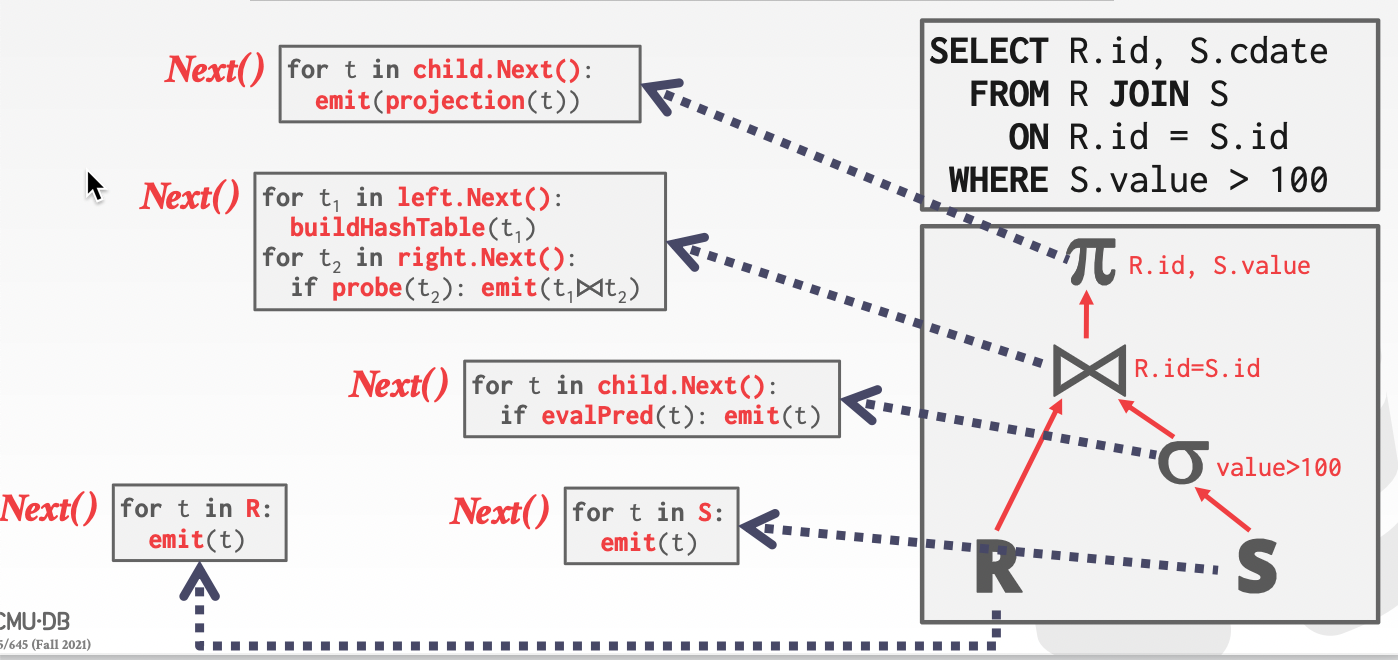
\includegraphics[width=.8\textwidth]{../images/15445/24.png}
\label{}
\end{figure}

This is used in almost every DBMS. Allows for tuple \textbf{pipelining}

some operators must block until their children emit all their tuples
\begin{itemize}
\item joins, subqueries, order by
\end{itemize}

output control works easily with this approach
\subsubsection{Materialization Model}
\label{sec:org407820a}
Each operator processes its input all at once and then emits its output all at once
\begin{itemize}
\item the operator ``materializes'' its output as a single result
\item the BDMS can push down hints (e.g. \texttt{LIMIT}) to avoid scaning too many tuples
\end{itemize}
\subsubsection{Vectorized/Batch Model}
\label{sec:orgb951e28}
\subsection{Access Methods}
\label{sec:org5617ccb}
\subsection{Modification Queries}
\label{sec:orgd4bf422}
\subsection{Expression Evaluation}
\label{sec:org4a97e44}
\end{document}
